% Chapter Template

\chapter{Deep style transfer for synthesis of images of CAR-T cell populations} % Main chapter title
\chaptermark{Deep style transfer}

\label{Chapter6} % Change X to a consecutive number; for referencing this chapter elsewhere, use \ref{ChapterX}

\textbf{Summary}: \emph{The previous chapter illustrated the limitations of an automatically-generated training set for phenotyping cells in CAR-T experiments, whose accuracy degrades over time with fluorescent quenching. This final chapter formalises and tests novel ideas for circumventing these limitations. An approach based in style transfer is proposed for synthesising cell line populations according to user-defined content by leveraging unsupervised generative models. This succeeds in generating realistic phase contrast images with a complete ground truth sufficient to train a state-of-the-art object detection system.}

\textbf{R\'esum\'e}: \emph{Le chapitre pr\'ec\'edent a illustr\'e les limites des donn\'ees d'entra\^inement g\'en\'er\'ees automatiquement pour le ph\'enotypage des cellules dans les essais CAR-T, dont la pr\'ecision se d\'egrade avec le temps. Ce dernier chapitre formalise et teste de nouvelles id\'ees pour contourner ces limites. Une approche bas\'ee sur le transfert de style est propos\'ee pour synth\'etiser des populations de lign\'ees cellulaires selon une sp\'ecification de contenu d\'efinie par l'utilisateur en s'appuyant sur des mod\`eles g\'en\'eratifs non supervis\'es. Cela permet de g\'en\'erer des images r\'ealistes \`a contraste de phase avec une annotation compl\`ete suffisante pour entra\^iner un syst\`eme de d\'etection d'objets de pointe.}

\section{Overview}

Chapter \ref{Chapter5} compared approaches for detecting and classifying cell types from phase contrast images: directly using an object detection system; and indirectly using a fluorescence predictor (which doubles as a visualisation tool). Each approach had its shortcomings: highly clustered cells prevent the harvesting of training data for object detection, and fluorescent quenching in later experimental frames caused problems for both. In this chapter we explore an entirely different approach that aims to circumvent these problems. This approach is based on generative models.

The desired end result is an endless supply of perfectly annotated synthetic images, on which we can train a state-of-the-art object detector. The intention is that such a detector will transfer seamlessly to the true data and outperform the Chapter \ref{Chapter5} approaches. In that chapter, a custom object detection system was designed to be trainable without a full annotation of the data. With a full annotation, the options for detector are broadened considerably.

%By application of Bayes' theorem it can be shown for latent variables $\mathbf{z}$ and generated variables $\mathbf{x}$ that,
%
%$$\log p_\theta(\mathbf{x}^{(i)}) = D_{KL}\big(q_\phi(\mathbf{z}|\mathbf{x}^{(i)}) || p_\theta(\mathbf{z}|\mathbf{x}^{(i)}) \big) + \underbrace{\mathbb{E}_{q_\phi(\mathbf{z}|\mathbf{x})}
%\bigg[\log \frac{p_\theta(\mathbf{x}^{(i)}, \mathbf{z})}{q_\phi(\mathbf{z}|\mathbf{x}^{(i)})}\bigg]}_{\mathcal{L}(\theta, \phi ; \mathbf{x}^{(i)})}$$
%
%We drop the divergence term, which is non-negative, and optimise the lower bound, $\log p_\theta(\mathbf{x}^{(i)}) \geq \mathcal{L}(\theta, \phi ; \mathbf{x}^{(i)})$. With a reparameterisation of the distribution on $\mathbf{z}$, one gets the stochastic gradient variational Bayes (SVGB) estimator, and the corresponding and eponymous auto-encoding variational Bayes (AEVB) optimisation algorithm (gradient descent with Monte Carlo sampling). This function can be rewritten as,
%
%$$\mathcal{L}(\theta, \phi ; \mathbf{x}^{(i)}) = -D_{KL}\big(q_\phi(\mathbf{z}|\mathbf{x}^{(i)}) || p_\theta(\mathbf{z}) \big) + \mathbb{E}_{q_\phi(\mathbf{z}|\mathbf{x})} \big[\log p_\theta(\mathbf{x}^{(i)}| \mathbf{z})\big]$$
%
%A further simplification can then be reached by choosing conjugate distributions (here decorrelated Gaussians) for $q_\phi(\mathbf{z}|\mathbf{x}^{(i)})$ and $p_\theta(\mathbf{z})$, yielding an \emph{analytic simplification} of the divergence term. This leaves the expectation to be optimised with sampling. The distribution $p_\theta(\mathbf{x}^{(i)}| \mathbf{z})$ is also chosen to be a decorrelated Gaussian. The parameters for the encoding and decoding distributions are predicted by respective neural networks (in the paper, MLPs with single hidden layers). The likelihood function, optimised with gradient ascent, is then,
%
%$$\mathcal{L}(\theta, \phi ; \mathbf{x}^{(i)}) = \frac{1}{2}\sum_{j=1}^J\Big(1 + \log((\sigma_j^{(i)})^2) - (\mu_j^{(i)})^2 - (\sigma_j^{(i)})^2\Big) + \frac{1}{L}\sum_{l=1}^L\log p_{\theta}(\mathbf{x}^{i}|\mathbf{z}^{(i, l)})$$
%
%where the left-hand sum (akin to a regulariser) comes from the simplification on the divergence term (from the choice of Gaussians) and the right-hand term samples the encoder. In practice, as we will optimise with mini-batch gradient descent, a single sample is used ($L = 1$). If this decoder distribution is chosen to be Gaussian (real-valued), the log probability becomes a mean-square loss; if the distribution is binomial (binary-valued), it becomes a binary cross-entropy loss\footnote{As in the Chollet demo, which is also why no variance vector is predicted by the decoder network--the variance is equal to the mean in a binomial distribution (or rather because we simply take the mean as our sample anyway?).}. The system is optimsed end-to-end: mini-batches of $\mathbf{x}$ are sampled from the ground truth, a distribution on each latent variable $\mathbf{z}$ is produced, from which we sample $L$ times. For each, we produce a distribution on the decoded variable, from which we take the mean. This results in a loss function in terms of the parameters of the neural networks (see above).
%
%\begin{figure}
%\begin{center}
%\tikzset{every picture/.style={line width=0.75pt}} %set default line width to 0.75pt        
%
%\begin{tikzpicture}[x=0.75pt,y=0.75pt,yscale=-1,xscale=1]
%%uncomment if require: \path (0,205); %set diagram left start at 0, and has height of 205
%
%%Straight Lines [id:da5482506046950146] 
%\draw    (185,11) -- (190,11) ;
%
%
%%Straight Lines [id:da12987643255151193] 
%\draw    (185,61) -- (190,61) ;
%
%
%%Straight Lines [id:da4195778005918448] 
%\draw    (190,61) -- (190,11) ;
%
%
%%Straight Lines [id:da7261947265305708] 
%\draw    (190,36) -- (195,36) ;
%
%%Straight Lines [id:da3894152295795107] 
%\draw    (40,16) -- (70,26) ;
%
%
%%Straight Lines [id:da9140322835321197] 
%\draw    (40,16) -- (70,46) ;
%
%
%%Straight Lines [id:da0009514658444130797] 
%\draw    (40,26) -- (70,26) ;
%
%
%%Straight Lines [id:da5552552447304977] 
%\draw    (40,26) -- (70,46) ;
%
%
%%Straight Lines [id:da9509018466715194] 
%\draw    (40,16) -- (70,36) ;
%
%
%%Straight Lines [id:da8581155992784358] 
%\draw    (40,26) -- (70,36) ;
%
%
%%Straight Lines [id:da8088246875536318] 
%\draw    (40,36) -- (70,26) ;
%
%
%%Straight Lines [id:da5571353494207303] 
%\draw    (40,36) -- (70,36) ;
%
%
%%Straight Lines [id:da4858891776431381] 
%\draw    (40,36) -- (70,46) ;
%
%
%%Straight Lines [id:da8785838787095616] 
%\draw    (40,46) -- (70,26) ;
%
%
%%Straight Lines [id:da8003432626318989] 
%\draw    (40,46) -- (70,36) ;
%
%
%%Straight Lines [id:da6602403280932999] 
%\draw    (40,46) -- (70,46) ;
%
%
%%Straight Lines [id:da7852830801220664] 
%\draw    (40,56) -- (70,26) ;
%
%
%%Straight Lines [id:da3338953157193171] 
%\draw    (40,56) -- (70,36) ;
%
%
%%Straight Lines [id:da96410539003723] 
%\draw    (40,56) -- (70,46) ;
%
%
%%Straight Lines [id:da37657353813646166] 
%\draw    (80,26) -- (110,16) ;
%
%
%%Straight Lines [id:da24128597928899576] 
%\draw    (80,26) -- (110,26) ;
%
%
%%Straight Lines [id:da32547027440752274] 
%\draw    (80,36) -- (110,16) ;
%
%
%%Straight Lines [id:da31170209674818405] 
%\draw    (80,36) -- (110,26) ;
%
%
%%Straight Lines [id:da27746879669185276] 
%\draw    (80,46) -- (110,16) ;
%
%
%%Straight Lines [id:da09414464198209282] 
%\draw    (80,46) -- (110,26) ;
%
%
%%Straight Lines [id:da8001404977472554] 
%\draw    (80,46) -- (110,46) ;
%
%
%%Straight Lines [id:da21073882551792977] 
%\draw    (80,46) -- (110,56) ;
%
%
%%Straight Lines [id:da14544461589198465] 
%\draw    (80,26) -- (110,46) ;
%
%
%%Straight Lines [id:da6238707251021953] 
%\draw    (80,26) -- (110,56) ;
%
%
%%Straight Lines [id:da367572619806544] 
%\draw    (80,36) -- (110,46) ;
%
%
%%Straight Lines [id:da7376946175347324] 
%\draw    (80,36) -- (110,56) ;
%
%
%%Shape: Circle [id:dp6891535439236647] 
%\draw   (30,16) .. controls (30,13.24) and (32.24,11) .. (35,11) .. controls (37.76,11) and (40,13.24) .. (40,16) .. controls (40,18.76) and (37.76,21) .. (35,21) .. controls (32.24,21) and (30,18.76) .. (30,16) -- cycle ;
%%Shape: Circle [id:dp4809043139793967] 
%\draw   (40,56) .. controls (40,53.24) and (37.76,51) .. (35,51) .. controls (32.24,51) and (30,53.24) .. (30,56) .. controls (30,58.76) and (32.24,61) .. (35,61) .. controls (37.76,61) and (40,58.76) .. (40,56) -- cycle ;
%%Shape: Circle [id:dp8584070024461332] 
%\draw   (40,46) .. controls (40,43.24) and (37.76,41) .. (35,41) .. controls (32.24,41) and (30,43.24) .. (30,46) .. controls (30,48.76) and (32.24,51) .. (35,51) .. controls (37.76,51) and (40,48.76) .. (40,46) -- cycle ;
%%Shape: Circle [id:dp276696925378514] 
%\draw   (40,26) .. controls (40,23.24) and (37.76,21) .. (35,21) .. controls (32.24,21) and (30,23.24) .. (30,26) .. controls (30,28.76) and (32.24,31) .. (35,31) .. controls (37.76,31) and (40,28.76) .. (40,26) -- cycle ;
%%Shape: Circle [id:dp5068716420834293] 
%\draw   (40,36) .. controls (40,33.24) and (37.76,31) .. (35,31) .. controls (32.24,31) and (30,33.24) .. (30,36) .. controls (30,38.76) and (32.24,41) .. (35,41) .. controls (37.76,41) and (40,38.76) .. (40,36) -- cycle ;
%%Shape: Circle [id:dp25861297333334865] 
%\draw   (110,46) .. controls (110,43.24) and (112.24,41) .. (115,41) .. controls (117.76,41) and (120,43.24) .. (120,46) .. controls (120,48.76) and (117.76,51) .. (115,51) .. controls (112.24,51) and (110,48.76) .. (110,46) -- cycle ;
%%Shape: Circle [id:dp4643023392023927] 
%\draw   (120,56) .. controls (120,53.24) and (117.76,51) .. (115,51) .. controls (112.24,51) and (110,53.24) .. (110,56) .. controls (110,58.76) and (112.24,61) .. (115,61) .. controls (117.76,61) and (120,58.76) .. (120,56) -- cycle ;
%%Shape: Circle [id:dp49483512207009894] 
%\draw   (120,26) .. controls (120,23.24) and (117.76,21) .. (115,21) .. controls (112.24,21) and (110,23.24) .. (110,26) .. controls (110,28.76) and (112.24,31) .. (115,31) .. controls (117.76,31) and (120,28.76) .. (120,26) -- cycle ;
%%Shape: Circle [id:dp6189196673866093] 
%\draw   (120,16) .. controls (120,13.24) and (117.76,11) .. (115,11) .. controls (112.24,11) and (110,13.24) .. (110,16) .. controls (110,18.76) and (112.24,21) .. (115,21) .. controls (117.76,21) and (120,18.76) .. (120,16) -- cycle ;
%%Shape: Circle [id:dp26334938397542296] 
%\draw   (70,26) .. controls (70,23.24) and (72.24,21) .. (75,21) .. controls (77.76,21) and (80,23.24) .. (80,26) .. controls (80,28.76) and (77.76,31) .. (75,31) .. controls (72.24,31) and (70,28.76) .. (70,26) -- cycle ;
%%Shape: Circle [id:dp21117289762799085] 
%\draw   (80,36) .. controls (80,33.24) and (77.76,31) .. (75,31) .. controls (72.24,31) and (70,33.24) .. (70,36) .. controls (70,38.76) and (72.24,41) .. (75,41) .. controls (77.76,41) and (80,38.76) .. (80,36) -- cycle ;
%%Shape: Circle [id:dp6986281232195524] 
%\draw   (80,46) .. controls (80,43.24) and (77.76,41) .. (75,41) .. controls (72.24,41) and (70,43.24) .. (70,46) .. controls (70,48.76) and (72.24,51) .. (75,51) .. controls (77.76,51) and (80,48.76) .. (80,46) -- cycle ;
%%Shape: Circle [id:dp9465099631838082] 
%\draw   (40,136) .. controls (40,133.24) and (37.76,131) .. (35,131) .. controls (32.24,131) and (30,133.24) .. (30,136) .. controls (30,138.76) and (32.24,141) .. (35,141) .. controls (37.76,141) and (40,138.76) .. (40,136) -- cycle ;
%%Shape: Circle [id:dp0317784761129396] 
%\draw   (40,146) .. controls (40,143.24) and (37.76,141) .. (35,141) .. controls (32.24,141) and (30,143.24) .. (30,146) .. controls (30,148.76) and (32.24,151) .. (35,151) .. controls (37.76,151) and (40,148.76) .. (40,146) -- cycle ;
%%Straight Lines [id:da9071408874591911] 
%\draw    (40,136) -- (70,131) ;
%
%
%%Straight Lines [id:da24018419487947296] 
%\draw    (70,141) -- (40,136) ;
%
%
%%Straight Lines [id:da2197851178000082] 
%\draw    (70,151) -- (40,136) ;
%
%
%%Straight Lines [id:da22278232875335124] 
%\draw    (70,131) -- (40,146) ;
%
%
%%Straight Lines [id:da5286416322588332] 
%\draw    (70,141) -- (40,146) ;
%
%
%%Straight Lines [id:da9686539012443439] 
%\draw    (70,151) -- (40,146) ;
%
%
%%Straight Lines [id:da19068301978372293] 
%\draw    (80,131) -- (110,91) ;
%
%
%%Straight Lines [id:da7880914645247521] 
%\draw    (80,131) -- (110,101) ;
%
%
%%Straight Lines [id:da3700659225801386] 
%\draw    (80,131) -- (110,111) ;
%
%
%%Straight Lines [id:da47161960970243944] 
%\draw    (80,131) -- (110,121) ;
%
%
%%Straight Lines [id:da1890861259547718] 
%\draw    (80,131) -- (110,131) ;
%
%
%%Straight Lines [id:da68575440449275] 
%\draw    (80,141) -- (110,91) ;
%
%
%%Straight Lines [id:da3750607343399084] 
%\draw    (80,141) -- (110,101) ;
%
%
%%Straight Lines [id:da565282846349721] 
%\draw    (80,141) -- (110,111) ;
%
%
%%Straight Lines [id:da09138945664655973] 
%\draw    (80,141) -- (110,121) ;
%
%
%%Straight Lines [id:da6291765141176212] 
%\draw    (80,141) -- (110,131) ;
%
%
%%Straight Lines [id:da17649952679040037] 
%\draw    (80,151) -- (110,91) ;
%
%
%%Straight Lines [id:da9040253484064976] 
%\draw    (80,151) -- (110,101) ;
%
%
%%Straight Lines [id:da319584223894385] 
%\draw    (80,151) -- (110,111) ;
%
%
%%Straight Lines [id:da6424110207536109] 
%\draw    (80,151) -- (110,121) ;
%
%
%%Straight Lines [id:da48301959183093235] 
%\draw    (80,151) -- (110,131) ;
%
%
%%Straight Lines [id:da5808868333038631] 
%\draw    (80,151) -- (110,151) ;
%
%
%%Straight Lines [id:da10862128632113477] 
%\draw    (80,151) -- (110,161) ;
%
%
%%Straight Lines [id:da33295467729135] 
%\draw    (80,151) -- (110,171) ;
%
%
%%Straight Lines [id:da5943183168329922] 
%\draw    (80,151) -- (110,181) ;
%
%
%%Straight Lines [id:da49814525594220627] 
%\draw    (80,151) -- (110,191) ;
%
%
%%Straight Lines [id:da5282188881640719] 
%\draw    (80,131) -- (110,151) ;
%
%
%%Straight Lines [id:da8223632943255978] 
%\draw    (80,131) -- (110,161) ;
%
%
%%Straight Lines [id:da7243623571618915] 
%\draw    (80,131) -- (110,171) ;
%
%
%%Straight Lines [id:da7261719054165141] 
%\draw    (80,131) -- (110,181) ;
%
%
%%Straight Lines [id:da39705793171673787] 
%\draw    (80,131) -- (110,191) ;
%
%
%%Straight Lines [id:da18537995122881212] 
%\draw    (80,141) -- (110,151) ;
%
%
%%Straight Lines [id:da45329055012421227] 
%\draw    (80,141) -- (110,161) ;
%
%
%%Straight Lines [id:da5225449624979573] 
%\draw    (80,141) -- (110,171) ;
%
%
%%Straight Lines [id:da32195889549848067] 
%\draw    (80,141) -- (110,181) ;
%
%
%%Straight Lines [id:da9391190553840826] 
%\draw    (80,141) -- (110,191) ;
%
%
%%Shape: Circle [id:dp2915628817390813] 
%\draw   (110,151) .. controls (110,148.24) and (112.24,146) .. (115,146) .. controls (117.76,146) and (120,148.24) .. (120,151) .. controls (120,153.76) and (117.76,156) .. (115,156) .. controls (112.24,156) and (110,153.76) .. (110,151) -- cycle ;
%%Shape: Circle [id:dp5320512421785244] 
%\draw   (120,191) .. controls (120,188.24) and (117.76,186) .. (115,186) .. controls (112.24,186) and (110,188.24) .. (110,191) .. controls (110,193.76) and (112.24,196) .. (115,196) .. controls (117.76,196) and (120,193.76) .. (120,191) -- cycle ;
%%Shape: Circle [id:dp5934996363472481] 
%\draw   (120,181) .. controls (120,178.24) and (117.76,176) .. (115,176) .. controls (112.24,176) and (110,178.24) .. (110,181) .. controls (110,183.76) and (112.24,186) .. (115,186) .. controls (117.76,186) and (120,183.76) .. (120,181) -- cycle ;
%%Shape: Circle [id:dp4031144610077395] 
%\draw   (120,161) .. controls (120,158.24) and (117.76,156) .. (115,156) .. controls (112.24,156) and (110,158.24) .. (110,161) .. controls (110,163.76) and (112.24,166) .. (115,166) .. controls (117.76,166) and (120,163.76) .. (120,161) -- cycle ;
%%Shape: Circle [id:dp9787620981523663] 
%\draw   (120,171) .. controls (120,168.24) and (117.76,166) .. (115,166) .. controls (112.24,166) and (110,168.24) .. (110,171) .. controls (110,173.76) and (112.24,176) .. (115,176) .. controls (117.76,176) and (120,173.76) .. (120,171) -- cycle ;
%%Shape: Circle [id:dp4465533781992891] 
%\draw   (110,91) .. controls (110,88.24) and (112.24,86) .. (115,86) .. controls (117.76,86) and (120,88.24) .. (120,91) .. controls (120,93.76) and (117.76,96) .. (115,96) .. controls (112.24,96) and (110,93.76) .. (110,91) -- cycle ;
%%Shape: Circle [id:dp023823674924046356] 
%\draw   (120,131) .. controls (120,128.24) and (117.76,126) .. (115,126) .. controls (112.24,126) and (110,128.24) .. (110,131) .. controls (110,133.76) and (112.24,136) .. (115,136) .. controls (117.76,136) and (120,133.76) .. (120,131) -- cycle ;
%%Shape: Circle [id:dp33712354428314706] 
%\draw   (120,121) .. controls (120,118.24) and (117.76,116) .. (115,116) .. controls (112.24,116) and (110,118.24) .. (110,121) .. controls (110,123.76) and (112.24,126) .. (115,126) .. controls (117.76,126) and (120,123.76) .. (120,121) -- cycle ;
%%Shape: Circle [id:dp8548192014024346] 
%\draw   (120,101) .. controls (120,98.24) and (117.76,96) .. (115,96) .. controls (112.24,96) and (110,98.24) .. (110,101) .. controls (110,103.76) and (112.24,106) .. (115,106) .. controls (117.76,106) and (120,103.76) .. (120,101) -- cycle ;
%%Shape: Circle [id:dp7728001976398915] 
%\draw   (120,111) .. controls (120,108.24) and (117.76,106) .. (115,106) .. controls (112.24,106) and (110,108.24) .. (110,111) .. controls (110,113.76) and (112.24,116) .. (115,116) .. controls (117.76,116) and (120,113.76) .. (120,111) -- cycle ;
%%Shape: Circle [id:dp2304318416361859] 
%\draw   (70,131) .. controls (70,128.24) and (72.24,126) .. (75,126) .. controls (77.76,126) and (80,128.24) .. (80,131) .. controls (80,133.76) and (77.76,136) .. (75,136) .. controls (72.24,136) and (70,133.76) .. (70,131) -- cycle ;
%%Shape: Circle [id:dp5016140232991698] 
%\draw   (80,141) .. controls (80,138.24) and (77.76,136) .. (75,136) .. controls (72.24,136) and (70,138.24) .. (70,141) .. controls (70,143.76) and (72.24,146) .. (75,146) .. controls (77.76,146) and (80,143.76) .. (80,141) -- cycle ;
%%Shape: Circle [id:dp9161710801953123] 
%\draw   (80,151) .. controls (80,148.24) and (77.76,146) .. (75,146) .. controls (72.24,146) and (70,148.24) .. (70,151) .. controls (70,153.76) and (72.24,156) .. (75,156) .. controls (77.76,156) and (80,153.76) .. (80,151) -- cycle ;
%%Straight Lines [id:da44792564481932606] 
%\draw    (185,85) -- (190,85) ;
%
%
%%Straight Lines [id:da6251406678528818] 
%\draw    (185,195) -- (190,195) ;
%
%
%%Straight Lines [id:da7640190795483477] 
%\draw    (190,195) -- (190,85) ;
%
%
%%Straight Lines [id:da09558281837096161] 
%\draw    (190,141) -- (195,141) ;
%
%
%
%% Text Node
%\draw (18,35.5) node [scale=0.9]  {$\mathbf{x}$};
%% Text Node
%\draw (151,20.5) node [scale=0.9]  {$\mathbf{\mu }_{E}$};
%% Text Node
%\draw (152.5,49) node [scale=0.9]  {$\log\mathbf{\sigma }^{2}_{E}$};
%% Text Node
%\draw (277,36.5) node [scale=0.9]  {$q_{\phi }(\mathbf{z} |\mathbf{x}) =\mathcal{N}\left(\mathbf{z} ;\mathbf{\mu }_{E} ,\sigma ^{2}_{E}\mathbf{I}\right)$};
%% Text Node
%\draw (17,138.5) node   {$\tilde{\mathbf{z}}$};
%% Text Node
%\draw (151.5,111.5) node [scale=0.9]  {$\mathbf{\mu }_{D}$};
%% Text Node
%\draw (151.5,169) node [scale=0.9]  {$\log\mathbf{\sigma }^{2}_{D}$};
%% Text Node
%\draw (285,142) node [scale=0.9]  {$p_{\theta }(\mathbf{x} |\mathbf{z}) =\mathcal{N}\left(\mathbf{x} ;\mathbf{\mu }_{D} ,\sigma ^{2}_{D}\mathbf{I}\right)$};
%
%
%\end{tikzpicture}
%\end{center}
%\end{figure}

%This paper is truly impressive. The authors propose a training strategy for taking GANs to high resolution (up to $1024^2$ pixels). Training is done in stages, beginning at low resolutions ($4\times 4$), and increasing the resolution twofold at intervals. This is done simply by adding new layers to the generator and discriminator, which remain symmetric throughout training. To curtail the impact of adding new layers with random weights, the new layer is ``faded in'' with a residual collection, allowing it to simply perform the identity operation at first, before the skip connection is gradually turned off\footnote{This highlights the power of the residual block for facilitating learning in deep networks.}. Thus, the GAN learns global structures first at low resolution, and progressively refines its output. They find that this approach makes for faster learning than comparable approaches, which otherwise attempt to learn all structure (global and fine) at once. Note this is not a greedy optimisation, as all layers remain trainable throughout; the authors describe it rather as implicit curriculum learning (i.e. learning easy tasks first before ramping difficulty up).
%
%A major challenge is dealing with the necessarily smaller batch sizes of the high resolution inputs. For this, they devise a number of normalisation strategies. Other contributions of the paper include a new metric for better assessing variation in generator outputs (the crux is to compare with statistics from the training set). They also publish a new version of the CelebA dataset, CelebA-HQ ($1024^2$), on which they do the training. Despite the dazzling results, this consists of a mere 30,000 images!
%
%This paper proposes several autoregressive (AR) models for image generation. As a result, it is a very busy paper, and hard to follow every detail. The basic idea is to generate pixels one-by-one by conditioning on previously generated pixels in a structured context, using RNNs (PixelRNN) and also a fully-convolutional network (PixelCNN). Apart from image generation, one nice application is image imputation (completion) of occluded images. Due to their unorthodoxy, AR models are surely the dark horse of the ``big three'' deep generative models for images (along with GANs and VAEs), yet they seem to work surprisingly well.

\section{Feasibility study: synthesising cell crops}
\label{sec:feasibility_synthesising}

To assess the feasibility of using generative models for cell population generation, let us attack a simpler problem: generating crops of individual cells. There are grounds for optimism, given the low target resolution, coupled with the abundance of training data. \cite{osokin2017gans} earlier achieved impressive results synthesising fluorescence readouts of cell crops. Using the automatic cropping strategy detailed in Chapter \ref{Chapter5}, a training set of $42241$ $24 \times 24$px cell crops were assembled from four days of frames from the well A01, field $1$ (a Raji-only experiment). The natural imbalance of cell states produced a class imbalance of $32507$ living to $9734$ dead cells. Samples from the training set are given in Figure \ref{fig:reference_samples}.

\begin{figure}[h]
\centering
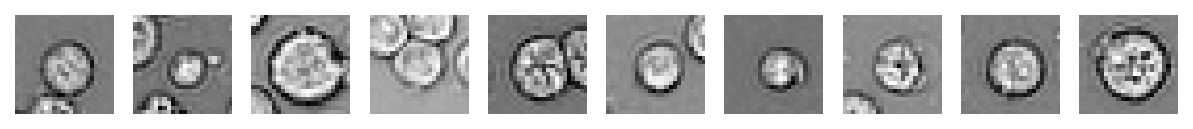
\includegraphics[width=\textwidth]{img/feasibility_reference_samples.pdf}
\caption{Example cell-centered $24\times 24$px crops from the ground truth training set.}
\label{fig:reference_samples}
\end{figure}

Fully-connected and deep convolutional GANs were trained, along with conditional versions of each (see Section \ref{sec:gans_definition} for an overview of GANs and see Appendix \ref{appendix:fcgan}, \ref{appendix:dcgan} for network specifications). In training the conditional models, the number of living and dead Raji cells sampled were balanced in each mini-batch. Otherwise, the training settings were held constant across the experiments: $50$ epochs; batch sizes of $120$ samples; $100$-dimensional Gaussian noise input. All models were trained with the Adam optimiser (\cite{kingma2014adam}) with maximum learning rate $2e^{4})$, $(\beta_0, \beta_1) = (0.5, 0.999)$, and learning rate decay $1e^{-6}$, with the Jensen-Shannon objective function.

\subsection{Generative adversarial networks}

The simplest practicable variant of GANs incorporates $D$ and $G$ as fully-connected networks. Such models, show (perhaps cherry-picked) success in generating MNIST digits in \cite{goodfellow2014generative}, which likewise are of low resolution. Figure \ref{fig:gan_samples} shows, however, underwhelming results sampled from the trained fully-connected generator, with only rudimentary intensity levels and cellular structure of the ground truth captured. Furthermore, difficulties with mode collapse were  encountered more frequently than when dealing with the convolutional variants below. This lends support to the presumption that there is little to recommend fully-connected GANs for computer vision applications.

\begin{figure}[h!]
\centering
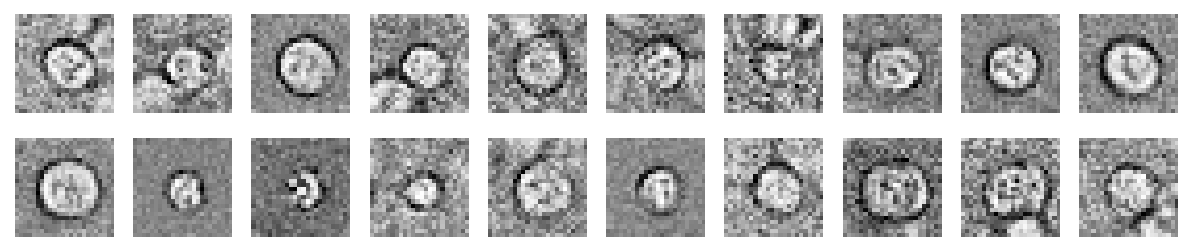
\includegraphics[width=\textwidth]{img/feasibility_gan_samples.pdf}
\caption{Sample $24\times 24$px crops from a fully-connected GAN.}
\label{fig:gan_samples}
\end{figure}

\subsection{Deep convolutional GANs}

Deep convolutional GANs (DCGANs) represent a vast improvement over the MLP-based GANs trained above. Figure \ref{fig:dcgan_samples} provides samples from the convolutional generator that are qualitatively close to ground truth samples\footnote{Indeed, when swapped with true samples, they succeeded in fooling a room full of experts as to their authenticity.}, with recognisable cellular characteristics, as well as convincing neighbouring cells in the crop periphery.

\begin{figure}[h!]
\centering
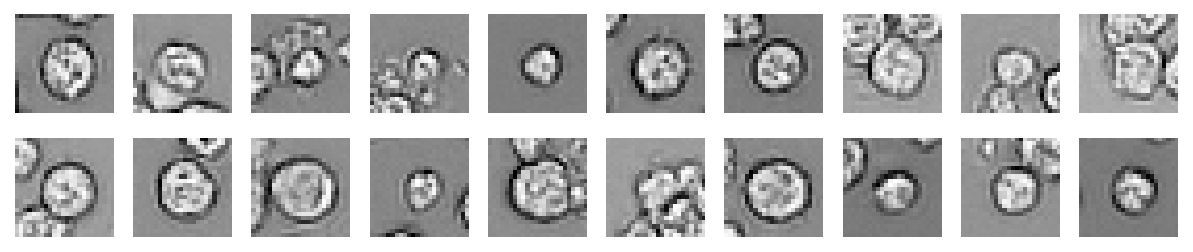
\includegraphics[width=\textwidth]{img/feasibility_dcgan_samples.pdf}
\caption{Sample $24\times 24$px crops from a DCGAN. One may notice the generator has learned to synthesise convincing peripheral cells.}
\label{fig:dcgan_samples}
\end{figure}

To establish the uniqueness of these samples,a k-nearest neighbour classifier (k-NN) ($k=9$) was trained to retrieve the closest samples (in Euclidean distance) within the training data. Such a test is important, as one does not wish the network merely to memorise ground truth samples. A set of comparisons are made in Figure \ref{fig:knn_gan}, illustrating the absence of sample ``memorisation''. Note, however, that this is neither an altogether reliable nor conclusive test: a Euclidean k-NN could easily be fooled by a ``parrot'' GAN that simply emitted memorised samples with intensities scaled, but this does not appear to be the case here.

\begin{figure}[h!]
\centering
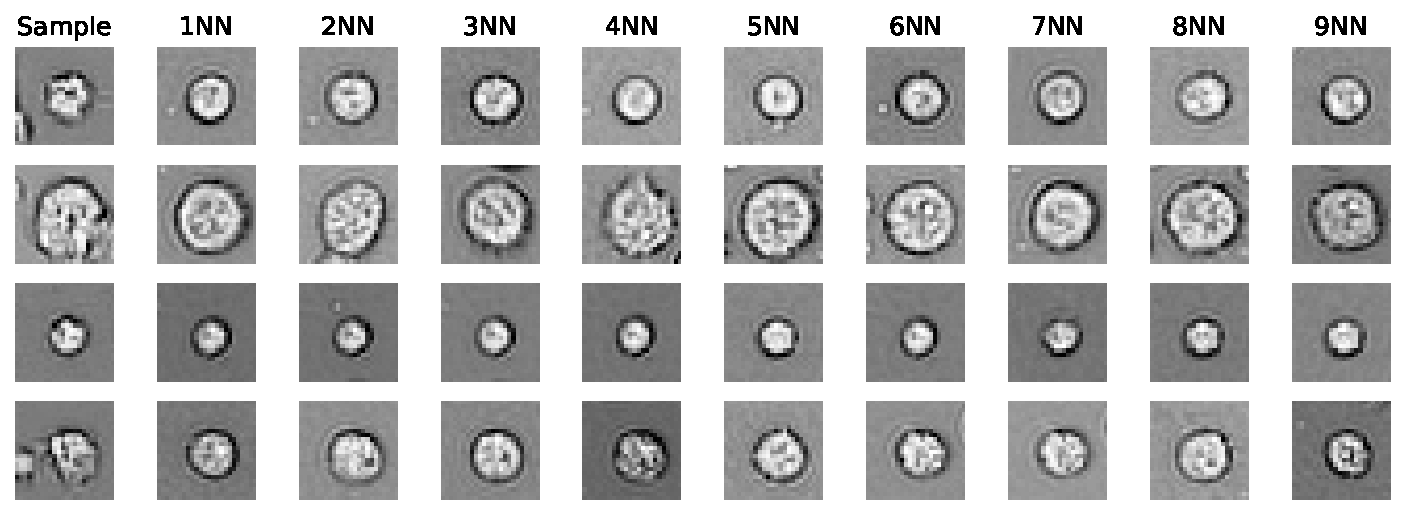
\includegraphics[width=\textwidth]{img/feasibility_knn_gan.pdf}
\caption{Comparison of cells generated with DCGAN (left-most column) against $9$ nearest neighbours from training set.}
\label{fig:knn_gan}
\end{figure}

\subsection{Conditional GANs}

Fully-connected and deep convolutional variants of CGANs are tried, where conditioning is made on class information for living and dead Raji cells. This is encoded as a two-dimensional one-hot vector. Note that this represents a first attempt to control the data generation process. As with the previous results with GANs, the results with fully-connected networks are underwhelming, and they are omitted from the discussion. Figure \ref{fig:cdcgan_samples}, however, displays samples from a conditional DCGAN, which are qualitatively both as convincing as our DCGAN samples, and also obey the conditional class signal, enabling on-demand generation of $10$ samples apiece for the two classes.

\begin{figure}[h!]
\centering
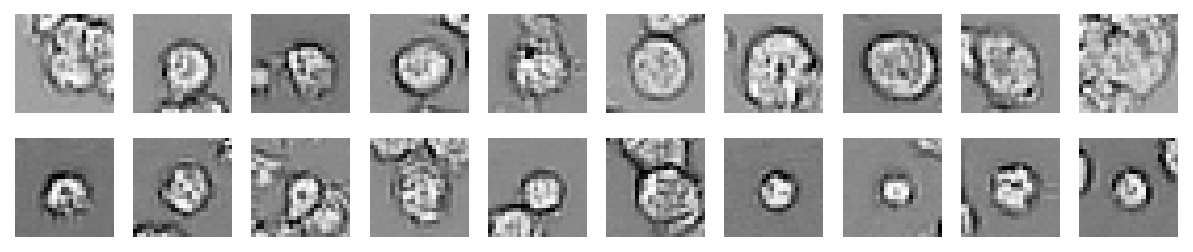
\includegraphics[width=\textwidth]{img/feasibility_cdcgan_samples.pdf}
\caption{Sample $24\times 24$px crops from a conditional DCGAN. The top row are crops produced by conditioning for living Raji cells; the bottom are crops produced by conditioning for dead Raji cells.}
\label{fig:cdcgan_samples}
\end{figure}

\section{Style transfer for simulating populations of Raji cells}
\label{subsec:style_transfer_application}

\cite{gatys2016image} proposed a ``neural algorithm of artistic style'', an algorithm to perform \emph{style transfer} using neural networks, the synthesis of an image combining textures of one style image and another content image. Note that this involved neither the architecting nor the training of a new purpose-built neural network, rather the clever utilisation of (any) pre-trained CNN. The work combined two related ideas: content reconstruction and texture reconstruction using CNNs. \textbf{Content reconstruction} with deep networks has been explored since the very first wave of CNNs assumed their primacy. \cite{zeiler2014visualizing} showed how their earlier ``deconvolutional network'' (\cite{zeiler2010deconvolutional}) could be used to reconstruct input images from the activations inside CNNs\footnote{The work is best remembered for proposing ``ZF-Net'', a very modest modification of AlexNet, as well as using pre-trained CNNs as feature extractors for other models.). In so doing, the paper did a lot to demystify the feature hierarchies learned by deep CNNs.}. \cite{simonyan2013deep} proposed a gradient-based method for visualising learned features of a pretrained network. Thus, a randomly initialised image was transformed into a structured image by incrementally adding its (regularised) gradient with respect to a chosen neuron from the network, so as to maximise the activation of that neuron. The deepest neurons, those corresponding to semantic object classes, led to the synthesis of recognisable yet ethereal impressions of those class objects. The authors argued their technique roughly generalised that of \cite{zeiler2014visualizing}. \cite{mahendran2015understanding} took the idea of using neuron-to-image gradients to full image construction. This is the idea that later inspired neural style transfer: a target image is fed into a pre-trained CNN and the tensor of its activations recorded; a randomly initialised synthesis image is then fed into the network, producing its own activation; the synthesis image is updated using gradient descent so as to minimise the mean square error of its activation to that of the target. The outcome may be a near-perfect reconstruction of the image. \textbf{Texture reconstruction} with CNNs was achieved by the same authors of style transfer in \cite{gatys2015texture}, in a prelude to that later work. The principle is the same as \cite{mahendran2015understanding}, yet rather than to reconstruct an image from its activations directly, one reconstructs for statisical properties derived from those features, namely their Gram matrix. The principle is that two images sharing such features are identical from a textural perspective. The authors write,

\begin{quotation}
\emph{Textures are per definition stationary, so a texture model needs to be agnostic to spatial information. A summary statistic that discards the spatial information in the feature maps is given by the correlations between the responses of different features. These feature correlations are, up to a constant of proportionality, given by the Gram matrix.}
\end{quotation}

In \cite{gatys2016image}, the ideas of style and content reconstruction were combined. Thus, one elects style $\mathbf{s}$ and content $\mathbf{c}$ reference images, and simultaneously reconstructs gradient-based reconstructions of a randomly initialised image $\mathbf{x}$,

\begin{align}
\mathcal{L}(\mathbf{s}, \mathbf{c}, \mathbf{x}) = \alpha\cdot\mathcal{L}_{\text{content}}(\mathbf{c}, \mathbf{x}) + \beta\cdot\mathcal{L}_{\text{style}}(\mathbf{s},\mathbf{x}),
\end{align}

for tunable weights $\alpha$ and $\beta$ and where the content loss,

\begin{align}
\mathcal{L}_{\text{content}}(\mathbf{c}, \mathbf{x}) = \frac{1}{2}||F^{(c)}(\mathbf{c}) - F^{(c)}(\mathbf{x})||_F^2,
\end{align}

for the vectorised $c$th layer (chosen by the programmer) of the pretrained network $F^{(c)} \in \mathbb{R}^{(N_cM_c \times K_c})$ with $N_c$, $M_c$, $K_c$ its dimensions, and the style loss,

\begin{equation}
\mathcal{L}_{\text{style}}(\mathbf{s}, \mathbf{x}) = \sum_{s \in S}\frac{1}{4N_s^2M_s^2}||G^{(s)}(\mathbf{c}) - G^{(s)}(\mathbf{x})||_F^2,
\label{eq:style_loss}
\end{equation}

where $G^{(s)} = F^{(s)}(F^{(s)})^T \in \mathbb{R}^{K \times K}$ is the Gram matrix of the matrix of vectorised feature maps $F^{(s)}$ of layer $s$. Note that the content reconstruction is usually performed on a single, deeper layer of the pretrained CNN, which is more invariant to style, while the style reconstruction can be performed at several shallower layers at once, to capture style at different scales. The result is a fusion of content and style in a synthesised image. An example is given in Figure \ref{fig:style_transfer}.

\begin{figure}%
    \centering
    \subfloat[Style]{{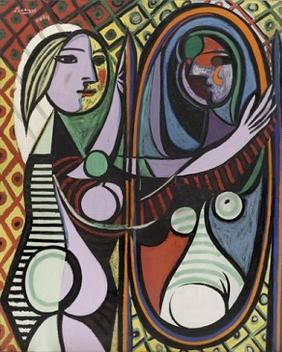
\includegraphics[height=0.35\textwidth]{img/picasso.jpg} }}%
    \qquad
    \subfloat[Content]{{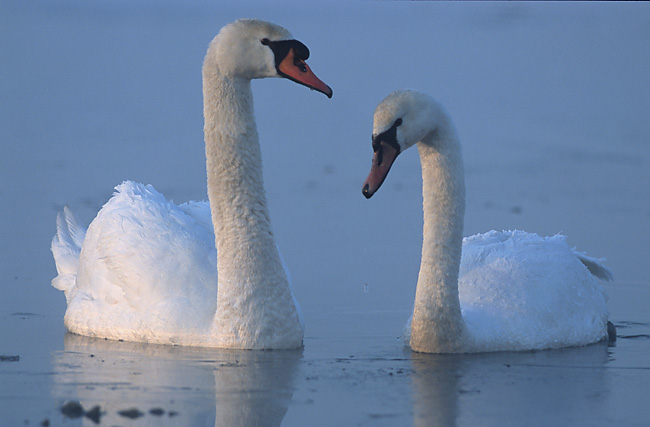
\includegraphics[height=0.35\textwidth]{img/swans.jpg} }}%
    \qquad
    \subfloat[Synthesis]{{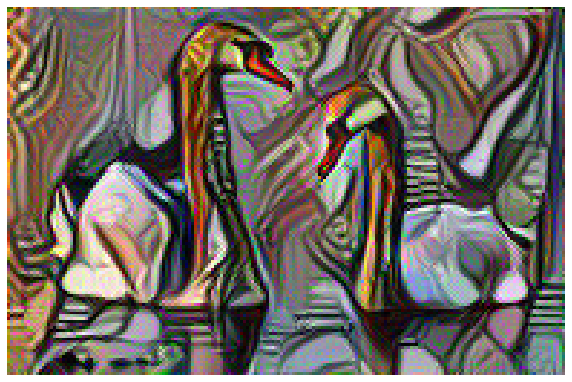
\includegraphics[height=0.35\textwidth]{img/style_transfer.png} }}
    \caption{A neural algorithm of artistic style uses a pretrained CNN to combine properties from a style source image (a) and a content source image (b) to synthesise a new image combining their characteristics (c). Example taken from https://github.com/jcboyd/vgg-fun}%
    \label{fig:style_transfer}%
\end{figure}

\subsection{Conditional dilation for tessellating cell contours}
\label{subsec:conditional_dilation}

Our objective is an application of style transfer to synthesise images of cells in phase contrast images from our CAR-T dataset. This is motivated from the shortcomings of the automatic training set extraction presented in Chapter \ref{Chapter5}, which provides an incomplete annotation of the data, and fails, crucially, in scenarios where cells cluster profusely, as in the case of strong proliferation. It was moreover found that this translated into the degradation of performance in time for both the fluorescence predictor and object detector. In principle, a perfectly annotated ground truth could be constructed using a style transfer procedure:

\begin{enumerate}
\item specify a desired content image by ``drawing'' content
\item manually crop a region of a phase contrast image with similar content
\item run the style transfer algorithm on the above
\end{enumerate}

Hypothetically, the outcome is a realistic-looking image of cells for which one has complete knowledge of its content, including cell position and size, thus the majority of information required for a fully-annotated object detection dataset (let us set aside the issue of class information for now), and indeed relates to the concept of data simulation. The idea of using style transfer for data augmentation has been shown to work in for example \cite{zheng2019stada}.

Given the simple geometric structure of cells, a good first approximation to a drawn cell is a circle. Therefore, in a space image plane $X$, the mask of an \emph{isolated} cell $k$ can be modeled as the set of points within distance $r_k$ to a non-empty set or ``site'' $P_k$,

\begin{equation}
R_k = \{x \in X | d(x, P_k) \leq r_k\},
\label{eq:region}
\end{equation}

where the distance $d(x, P_k) = \inf\{d(x, p) | p \in P_k\}$, that is, the shortest distance to any point in the site. When $P_k$ is a singleton set, the region becomes a circle. Otherwise, one may define the site $P_k$ in any way desired (for example, a line or eroded mask) to model random, anisotropic variations in cell shape. The radius,

\begin{align}
r_k \sim \mathcal{N}(\mu_i, \sigma_i),
\label{eq:radius_dist}
\end{align}

can be sampled from an estimation of the radius distribution for class $i$. Once again, let us avoid the complication of prescribing classes to cells for the present.

\begin{figure}%
    \centering
    \subfloat[\label{fig:voronoi}]{{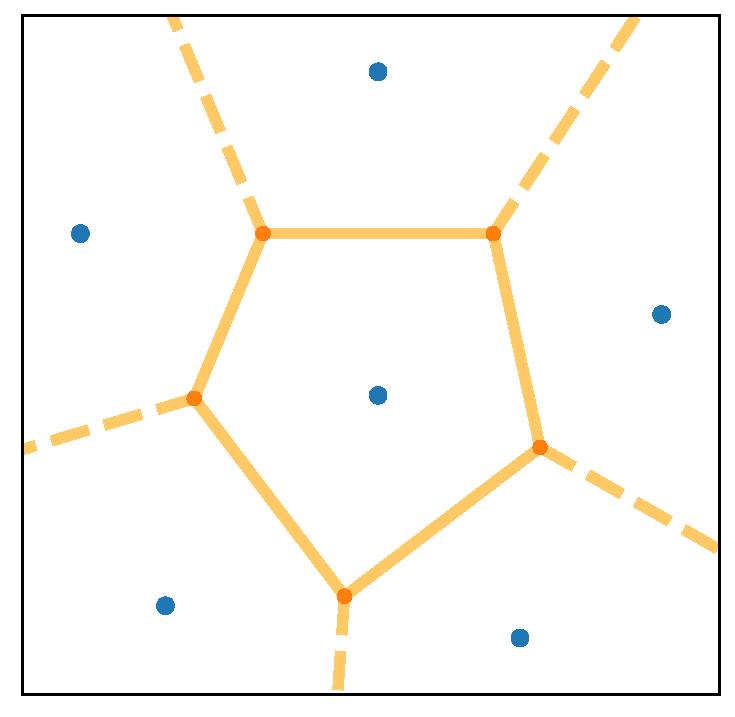
\includegraphics[width=0.25\textwidth]{img/voronoi.pdf} }}%
    \qquad
    \subfloat[\label{fig:cell_tessellation}]{{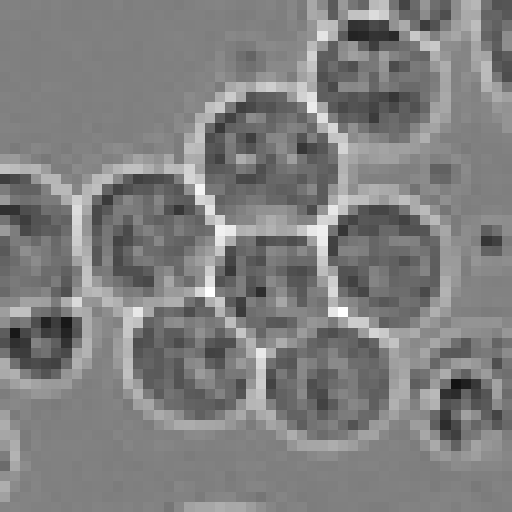
\includegraphics[width=0.25\textwidth]{img/tessellating_cells.png} }}
    \qquad
    \subfloat[]{{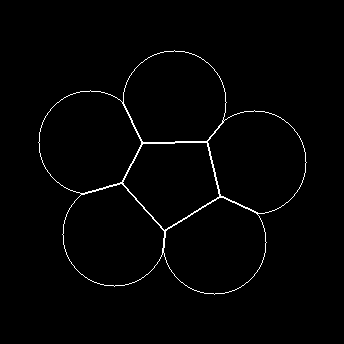
\includegraphics[width=0.25\textwidth]{img/conditional_dilation.png} }}
    \caption{Example of Voronoi tessellation with six sites (blue points) and corresponding regions (yellow lines) (generated in \texttt{scipy} (\cite{2020SciPy-NMeth}) (a). Neighbouring cells exhibit a tessellating effect at the border (b). A conditional dilation algorithm can model this bordering effect when it comes to synthesising content images for style transfer.}%
    \label{fig:conditional_dilation}%
\end{figure}

Though isolated cells are highly circular, closely neighbouring cells manifest a shared, flattened contour (see Figure \ref{fig:cell_tessellation}). Previously, \cite{bock2010generalized} have modeled the border forces of neighbouring cells as Voronoi-tessellating circles. A Voronoi tessellation can be defined as $K$ regions of the form,

\begin{equation}
S_k = \Big\{x \in X | d(x, P_k) \leq d(x, P_j) \forall j \neq k \Big\}.
\label{eq:voronoi}
\end{equation}

The $K$ regions constitute a partition of the space $X$, where points are assigned to the nearest site. An example is shown in Figure \ref{fig:voronoi} where a Euclidean distance is invoked for a set of six singleton sites. The borders between regions are lines perpendicular to the line joining the site centers. It is therefore proposed to model cells as the intersection of \ref{eq:region} and \ref{eq:voronoi},

\begin{equation}
T_k = \Big\{x \in X | d(x, P_k) \leq r_k \land d(x, P_k) \leq d(x, P_j) \  \forall j \neq k \Big\}.
\label{eq:conditional_dilation}
\end{equation}

%\begin{align}
%T_k &= R_k \cap S_k \\ \notag
%&= \Big\{x \in X | d(x, P_k) \leq r_k \land d(x, P_k) \leq d(x, P_j) \forall j \neq k \Big\}
%\end{align}

To compute the $T_k$, an algorithm for \emph{conditional dilation} is designed and shown in Algorithm \ref{alg:ConditionalDilation}. The principle is to select the sites (cell centres) and to grow outwards until either a maximum distance from the source is reached, or an object border is encountered. This resembles an implementation of the watershed algorithm, albeit with all seeds flooded from the same height (implemented as a priority of $0$). The dilation of sites is scheduled according to a priority queue, for which priority is assigned as the distance from the source\footnote{The \textsc{Dist} function for calculating minimum distances to the site sets implements a lookup table based on a pre-computed distance map.}. Thus, dilation propagates from the sites synchronously. The priority queue is implemented as a \emph{heap}, as it can push and pop in $\mathcal{O}(\log N)$ time.

\begin{algorithm}
\caption{Dilates labeled image SiteImage until distance from source exceeds Radii.} \label{alg:ConditionalDilation}
\begin{algorithmic}[1]
\Procedure{ConditionalDilation}{SiteImage, Radii}

\State PriorityQueue $\leftarrow$ \textsc{Heap}()

\For{marker in SiteImage}
    \State Elem $\leftarrow$ \textsc{HeapElement}()
    \State Elem.value $\leftarrow 0$ \Comment{Top priority}
    \State Elem.source $\leftarrow$ marker \Comment{Record origin}
    \State PriorityQueue.\textsc{Push}(Elem)
\EndFor

\While{$\lnot$ PriorityQueue.\textsc{IsEmpty}()}
    \State Elem $\leftarrow$ PriorityQueue.\textsc{Pop}()
    \For{Neighbour in Elem.\textsc{GetNeighbours}()}
        \If{SiteImage[Neighbour] $> 0$}
            \State \textbf{continue} \Comment{Neighbour already visited}
        \EndIf
        \State NewElem $\leftarrow$ \textsc{HeapElement}()
        \State NewElem.value $\leftarrow$ \textsc{Dist}(Neighbour, Elem.source)
        \If{NewElem.value $>$ Radii[Elem.source]} 
            \State \textbf{continue} \Comment{Cell border reached}
        \EndIf
        \State NewElem.source $\leftarrow$ Elem.source
        \State PriorityQueue.\textsc{Push}(NewElem)
        \State SiteImage[Neighbour] = SiteImage[Elem.source]
    \EndFor
\EndWhile
\State\Return SiteImage
\EndProcedure
\end{algorithmic}
\end{algorithm}

Applying this for the purpose of drawing cell population content images, the space $X$ becomes an image ``canvas'', that is, a two-dimensional array of numbers initialised to zero to indicate background. Sites are allocated as connected components (perhaps just points) of non-zero, foreground pixels. The canvas with its allocated sites and corresponding dilation radii are inputs to the \textsc{ConditionalDilation} algorithm. This works well in practice as long as the sites are carefully selected. For the time being, sites are chosen uniformly at random (without replacement)\footnote{One could imagine using a dynamically-updated distribution to simulate cell clustering.}, however sites must be chosen outside all other regions. Provided the canvas is large enough relative to the cells and the cell number, there is a large space of feasible allocations of sites. For efficiency, a record is kept of the vacant coordinates in the drawing canvas, from which is subtracted the coordinates of the anticipated region of each allocated site on-the-fly. If sites are naively allocated in arbitrary order, there is the risk of the scenario in which a larger cell is allocated in the vicinity of a smaller one, placing the center of the smaller cell within the region of the larger. A neat solution is to simply allocate the sites in descending order of radius. This procedure is described in Algorithm \ref{alg:AllocateSites}.

\begin{algorithm}
\caption{Allocates sites for input to \textsc{ConditionalDilation} algorithm. VacantCoords are a list of $(x, y)$ coordinates available for allocation (initially a full image), and Radii are the presampled radii for drawing cells.} \label{alg:AllocateSites}
\begin{algorithmic}[1]
\Procedure{AllocateSites}{VacantCoords, Radii}
% \State Let \emph{VacantCoords} be a list of coordinate tuples
\State Sites $\leftarrow$ []
\State Radii $\leftarrow$ \textsc{Sort}(Radii, descending=TRUE)

\For{radius in radii}
	\State Site $\leftarrow$ \textsc{Sample}(VacantCoords)
	\State Sites $\leftarrow$ Sites $\cup$ Site
	\State Region $\leftarrow \{$Coord $\in$ VacantCoords | $||$Coord - Site$||_2 <$ radius$\}$
	\State VacantCoords $\leftarrow$ VacantCoords $\setminus$ Region
\EndFor
\State\Return Sites
\EndProcedure
\end{algorithmic}
\end{algorithm}

The outcome of the \textsc{ConditionalDilation} algorithm is a content image in the form of a labeled mask. While masks are a natural choice for cell content markers, an alternative that is found to be more useful is the cell contour defined as,

\begin{equation}
C_k = T_k - T_k \oplus B_D,
\label{eq:contour}
\end{equation}

where $\oplus$ represents a morphological dilation or maximum filter, $T_k$ is the object mask, and $B_D$ is a (for example, disk-shaped) structuring element. The full procedure for generating content images is illustrated in Figure \ref{fig:conditional_dilation_process}.

\begin{figure}%
    \centering
    \subfloat[Points]{{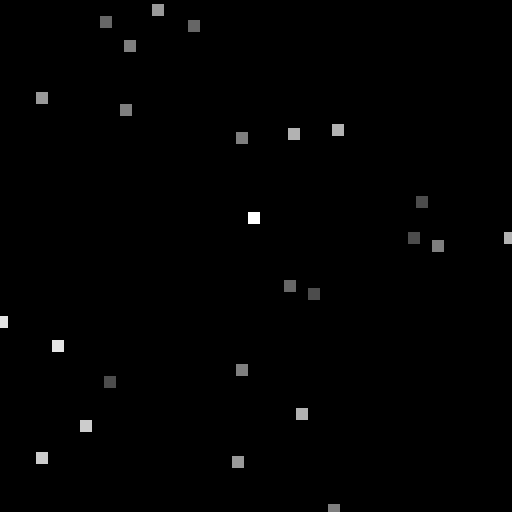
\includegraphics[width=0.25\textwidth]{img/cd_points.png}}}%
    \qquad
    \subfloat[Regions]{{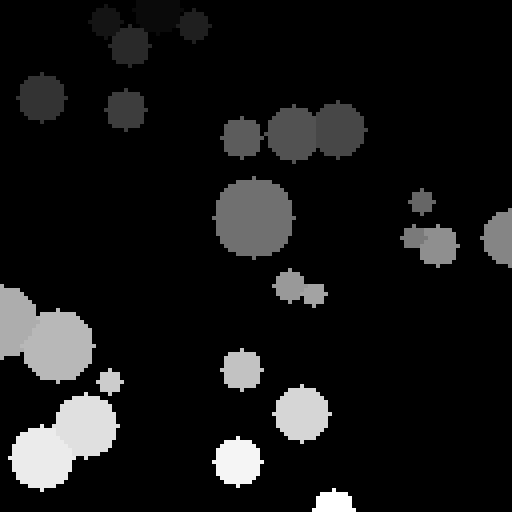
\includegraphics[width=0.25\textwidth]{img/cd_masks.png}}}%
    \qquad
    \subfloat[Contours]{{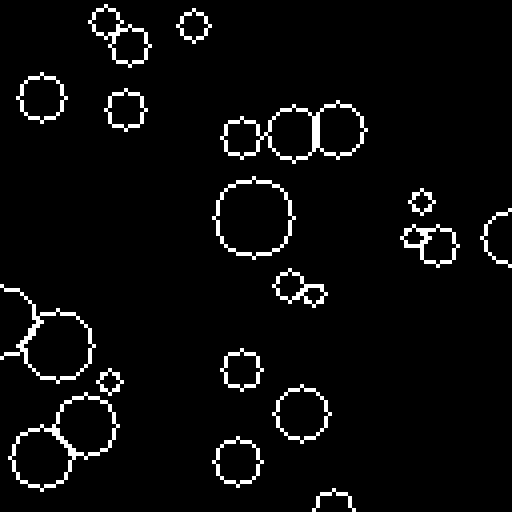
\includegraphics[width=0.25\textwidth]{img/cd_contours.png}}}%
    \caption{An example of generating a cell content image by first allocating sites with \textsc{AllocateSites} (a) (site intensity represents radius, dilated for visibility), with radii drawn from Equation \ref{eq:radius_dist}; running the \textsc{ConditionalDilation} algorithm to obtain labeled regions as in Equation \ref{eq:conditional_dilation} (b); and extracting the contours with Equation \ref{eq:contour} (c).}%
    \label{fig:conditional_dilation_process}
\end{figure}

\subsubsection{Results}

\begin{figure}[h]%
    \centering
    \subfloat[Style]{{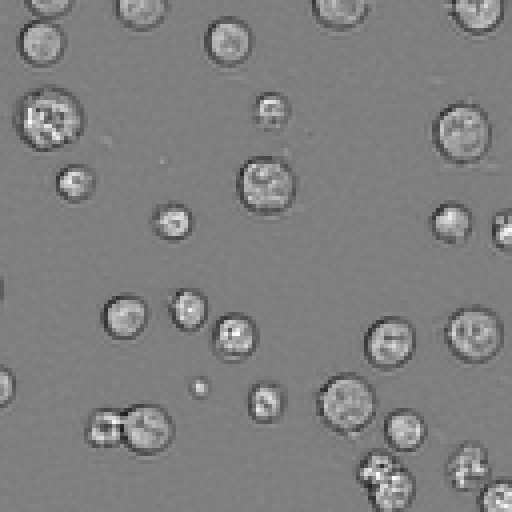
\includegraphics[width=0.25\textwidth]{img/style_style_img.png}}}%
    \qquad
    \subfloat[Content]{{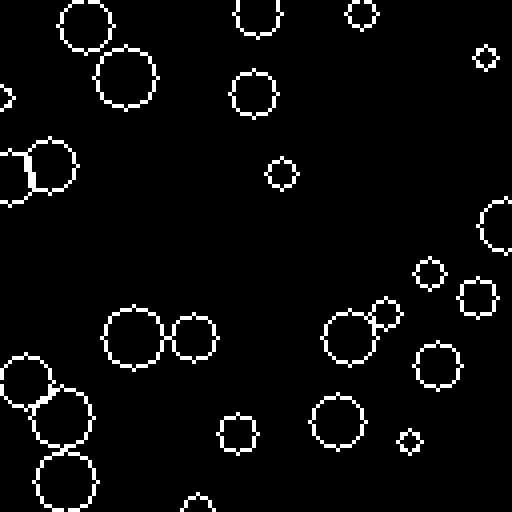
\includegraphics[width=0.25\textwidth]{img/style_content_img.png}}}%
    \qquad
    \subfloat[Synthesis]{{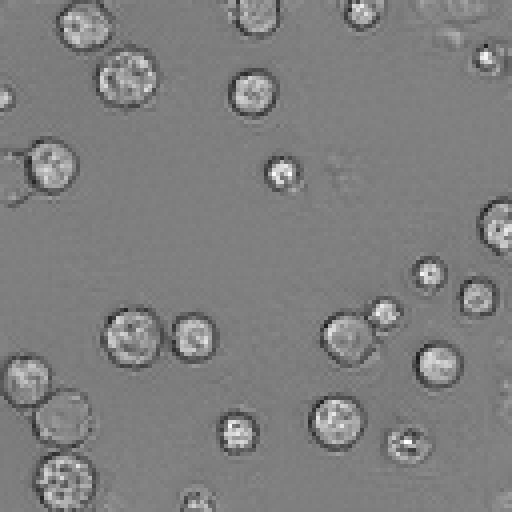
\includegraphics[width=0.25\textwidth]{img/style_synthesis_img.png}}}%
    \caption{An application of a neural algorithm of artistic style to phase contrast images of CAR-T cells (a) and a style source image (b) to synthesise a new image combining their characteristics in a ``simulated'' image (c).}%
    \label{fig:style_transfer_cells}
\end{figure}

Figure \ref{fig:style_transfer_cells} shows a first result with style transfer. The contours of cells are generated according to Equation \ref{eq:radius_dist}, which can be estimated from a library of pre-cropped cells from Chapter \ref{Chapter5}. The number of cells is chosen to match the chosen style image, and cells are placed uniformly randomly on the zeroed background plane. Here we see that the transfer succeeds--the background and foreground textures have been suitably apportioned to the objects prescribed by the content image. Various artifacts exist, of course, but individual cells appear correctly rendered, and the main fault is the global arrangement of the cell population lacking sense (recall objects have been placed uniformly randomly).

\begin{figure}%
    \centering
    \subfloat[Style]{{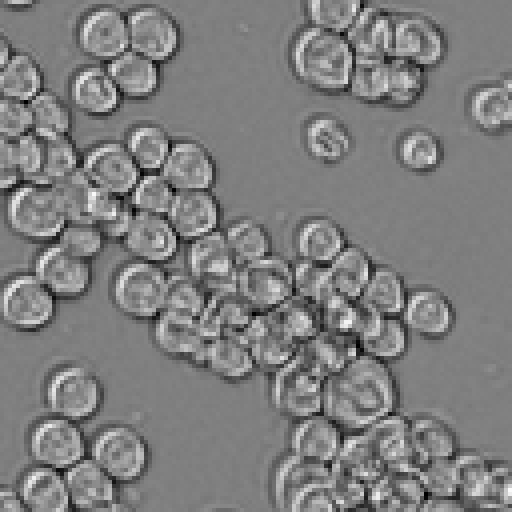
\includegraphics[width=0.25\textwidth]{img/style_style_img_many.png}}}%
    \qquad
    \subfloat[Content]{{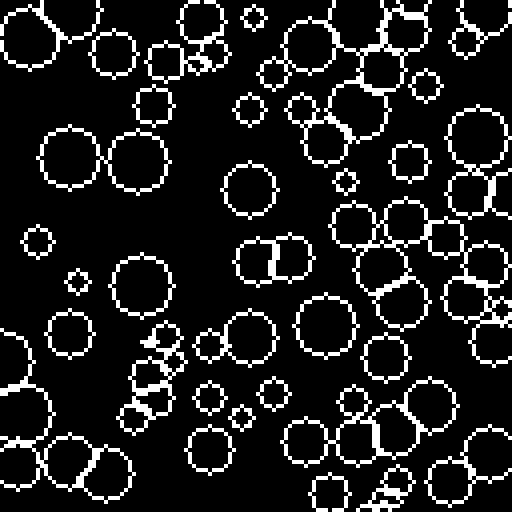
\includegraphics[width=0.25\textwidth]{img/style_content_img_many.png}}}%
    \qquad
    \subfloat[Synthesis]{{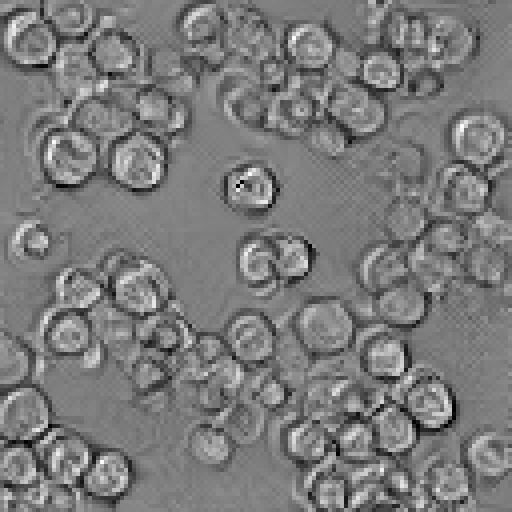
\includegraphics[width=0.25\textwidth]{img/style_synthesis_img_many.png}}}%
    \caption{More cells, more problems. The style transfer algorithm fails when the content image does not offer adequate ``scaffolding'' for the target texture patterns.}%
    \label{fig:style_transfer_cells_many}%
\end{figure}

Note that the low-resolution and simple geometric structure of the cells are naturally advantageous. Of course, if more complicated objects were to be modeled, the contour simulator need likewise be more sophisticated. There are, nevertheless, limitations to this approach. We see in Figure \ref{fig:style_transfer_cells_many} a larger population of cells with a greater degree of failure. In general, a tension is observed between the content specification and the chosen style crop. Note that Equation \ref{eq:style_loss} aims to ensure the same co-occurring neural activations invoked by the style target are invoked by the synthetic image also, albeit the global arrangement is arbitrary due to stationarity of the Gram matrix. The algorithm preferences applying these textures in the vicinity of recognisable contours, which is why one can steer the synthesis reasonably well. Furthermore, it is found that the cell geometry is flexible: when the disk contours are replaced with diamonds, for example, the algorithm still performs well. Yet, it is crucial to approximately match the size and number of cells between the style and content images to obtain a good distribution of texture. Indeed, the style image appears to provide a certain ``budget'' that if underspent will be apportioned arbitrarily (such as to the background), and if overspent will mean some objects end up untextured.

Though as a proof of concept this approach is successful and yields various insights, the pre-trained network, with all its particularities, does not offer the necessary control for bootstrapping a robust ground truth. In addition, the approach entails the manual curation of a suitable style reference image. What is more, the generation is slow: one must backprop a large neural network (although \cite{johnson2016perceptual} find ways of greatly improving the run time). To overcome these difficulties, in Section \ref{sec:cycle_gans} let us reformulate the problem as a learning problem of unsupervised image translation.

%\begin{algorithm}[H]
%\SetAlgoLined
%Let \emph{Open} by a priority queue\;
%Let \emph{Closed} have the same dimensions as \emph{DEM}\;
%Let \emph{Closed} be initialised to false\;
% \For{all c on the edges of \emph{DEM}}{
%  Push \emph{c} onto \emph{Open} with priority \emph{DEM}(\emph{c})\;
%  \emph{Closed}(\emph{c}) $\rightarrow$ TRUE
%  }
% \While{Open is not empty}{
%  \emph{c} $\rightarrow$ \textsc{POP}(Open)
%  \For{all neighbours n of c}{
%    \If{condition}{
%     continue;}
%  }
%  DEM(\emph{n} $\rightarrow$ \textsc{MAX}(DEM(\emph{n}), DEM(\emph{c}))\;
%  Closed(\emph{n}) $\rightarrow$ TRUE\;
%  Push \emph{n} onto Open with priority DEM(\emph{n})\;}
%  
%%  \eIf{condition}{
%%   instructions1\;
%%   instructions2\;
%%   }{
%%   instructions3\;
%%  }
%% }
% \caption{\textsc{Priority-Flood}: A generalization of the hierarchical-queue and priority-queue methods described by previous authors. Upon entry, (1) DEM contains the elevations of every cell or the value \textsc{NoData} for cells not part of the DEM. (2) The value \textsc{NoData} is less than the elevation of any cell. At exit,(1) DEM contains the elevations of every cell or the value \textsc{NoData} for cells not part of the DEM.(2) The elevations of DEM are such that there are no digital dams and no undrainable depressions in the landscape, though there may be flats. (\cite{barnes2014priority})}
%\label{alg:watershed}
%\end{algorithm}

%\begin{figure}%
%    \centering
%\tikzset{every picture/.style={line width=0.5pt}} %set default line width to 0.75pt        
%
%\begin{tikzpicture}[x=0.75pt,y=0.75pt,yscale=-1,xscale=1]
%%uncomment if require: \path (0,300); %set diagram left start at 0, and has height of 300
%
%%Image [id:dp4980478067048507] 
%\draw (132.25,136.08) node  {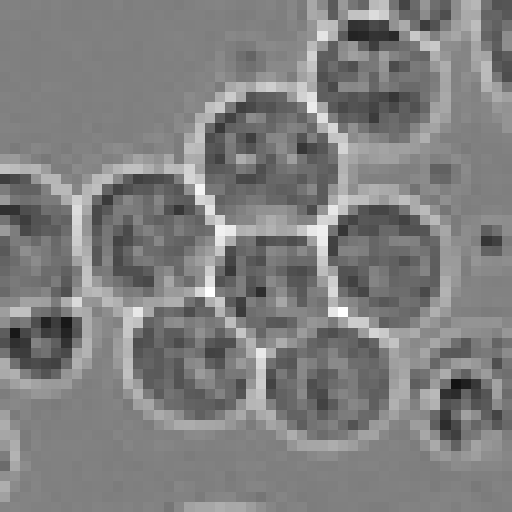
\includegraphics[width=196.88pt,height=196.88pt]{img/tessellating_cells.png}};
%%Straight Lines [id:da25370221998425035] 
%%Straight Lines [id:da25370221998425035] 
%%Straight Lines [id:da25370221998425035] 
%\draw [color={rgb, 255:red, 208; green, 2; blue, 27 }  ,draw opacity=1 ][line width=2.25]    (67.5,168.83) -- (107.5,154.83) ;
%%Curve Lines [id:da78429089295908] 
%\draw [color={rgb, 255:red, 208; green, 2; blue, 27 }  ,draw opacity=1 ][line width=2.25]    (134.5,213.83) .. controls (143.5,238.83) and (214.5,247) .. (200.5,179) ;
%%Straight Lines [id:da869721041867324] 
%\draw [color={rgb, 255:red, 208; green, 2; blue, 27 }  ,draw opacity=1 ][line width=2.25]    (43.17,111) -- (44.5,149.83) ;
%%Straight Lines [id:da606264756731195] 
%\draw [color={rgb, 255:red, 208; green, 2; blue, 27 }  ,draw opacity=1 ][line width=2.25]    (104.5,96.83) -- (115.5,124.83) ;
%%Curve Lines [id:da43862806357711237] 
%\draw [color={rgb, 255:red, 208; green, 2; blue, 27 }  ,draw opacity=1 ][line width=2.25]    (67.5,168.83) .. controls (57.5,229.83) and (108.5,234.83) .. (134.5,213.83) ;
%%Straight Lines [id:da007711051129161595] 
%\draw [color={rgb, 255:red, 208; green, 2; blue, 27 }  ,draw opacity=1 ][line width=2.25]    (134.5,182.83) -- (134.5,213.83) ;
%%Straight Lines [id:da8948759988905257] 
%\draw [color={rgb, 255:red, 208; green, 2; blue, 27 }  ,draw opacity=1 ][line width=2.25]    (107.5,154.83) -- (134.5,182.83) ;
%%Straight Lines [id:da559952041937628] 
%\draw [color={rgb, 255:red, 208; green, 2; blue, 27 }  ,draw opacity=1 ][line width=2.25]    (107.5,154.83) -- (115.5,124.83) ;
%%Straight Lines [id:da06843885355906787] 
%\draw [color={rgb, 255:red, 208; green, 2; blue, 27 }  ,draw opacity=1 ][line width=2.25]    (115.5,124.83) -- (165.5,122.83) ;
%%Straight Lines [id:da35300308696006066] 
%\draw [color={rgb, 255:red, 208; green, 2; blue, 27 }  ,draw opacity=1 ][line width=2.25]    (134.5,182.83) -- (170.5,163.83) ;
%%Straight Lines [id:da5353464045743885] 
%\draw [color={rgb, 255:red, 208; green, 2; blue, 27 }  ,draw opacity=1 ][line width=2.25]    (165.5,122.83) -- (170.5,163.83) ;
%%Straight Lines [id:da13390111475416988] 
%\draw [color={rgb, 255:red, 208; green, 2; blue, 27 }  ,draw opacity=1 ][line width=2.25]    (170.5,163.83) -- (200.5,179) ;
%%Curve Lines [id:da00783572797482568] 
%\draw [color={rgb, 255:red, 208; green, 2; blue, 27 }  ,draw opacity=1 ][line width=2.25]    (159.5,56) .. controls (139.5,32) and (90.5,61) .. (104.5,96.83) ;
%%Curve Lines [id:da46299196626045225] 
%\draw [color={rgb, 255:red, 208; green, 2; blue, 27 }  ,draw opacity=1 ][line width=2.25]    (175.5,76) .. controls (183.5,89) and (174.5,114) .. (170.5,113) ;
%%Curve Lines [id:da5311770081157473] 
%\draw [color={rgb, 255:red, 208; green, 2; blue, 27 }  ,draw opacity=1 ][line width=2.25]    (104.5,96.83) .. controls (78.5,84.83) and (56.5,85.83) .. (43.17,111) ;
%%Straight Lines [id:da0752881282120893] 
%\draw [color={rgb, 255:red, 208; green, 2; blue, 27 }  ,draw opacity=1 ][line width=2.25]    (44.5,149.83) -- (67.5,168.83) ;
%%Curve Lines [id:da9638447834881404] 
%\draw [color={rgb, 255:red, 208; green, 2; blue, 27 }  ,draw opacity=1 ][line width=2.25]    (200.5,179) .. controls (254.5,177) and (237.5,75) .. (170.5,113) ;
%%Straight Lines [id:da46356475878318215] 
%\draw [color={rgb, 255:red, 208; green, 2; blue, 27 }  ,draw opacity=1 ][line width=2.25]    (165.5,122.83) -- (170.5,113) ;
%%Straight Lines [id:da8863232629542646] 
%\draw [color={rgb, 255:red, 208; green, 2; blue, 27 }  ,draw opacity=1 ][line width=2.25]    (159.5,56) -- (175.5,76) ;
%\end{tikzpicture}
%
%\caption{A cluster of six Raji cells post mitosis. Cell membrane borders follow piecewise curves and, for the shared borders between neighbouring cells, straight line segments.}%
%    \label{fig:channels}%
%\end{figure}

\section{CycleGANs for cell population synthesis}
\label{sec:cycle_gans}

CycleGANs (\cite{isola2017image}) extend the \texttt{pix2pix} framework (see Section \ref{subsec:image_to_image}) to the \emph{unpaired} image-to-image translation setting, that is, translating between two (necessarily similar) image domains in a fully unsupervised way. Though the underlying neural network architectures remain virtually unchanged, the framework is quite different. CycleGANs introduce an additional pair of generator and discriminator. Now, one generator learns the mapping $G : X \to Y$ while the other learns $F : Y \to X$. The respective discriminators train these generators adversarially in the usual way. However, at the same time, there are cycle consistency losses ensuring $F(G(X)) \approx X$ (forward cycle consistency) and $G(F(Y)) \approx Y$ (backward cycle consistency). The cycle consistency loss,

\begin{equation}
\mathcal{L}_{CYC}(G, F) = \mathbb{E}_{x \sim p_{data}(x)}[||F(G(x)) - x||_1] + \mathbb{E}_{y \sim p_{data}(y)}[||G(F(y)) - y||_1],
\label{eq:cycle_consistency}
\end{equation}

that is, the expected $l_1$ error upon reconstructing real images via the stacked generators. Equation \ref{eq:cycle_consistency} is combined with the usual GAN losses for each direction of translation to give the CycleGAN objective,

\begin{equation}
\max_{G, F}\min_{D_X, D_Y} \mathcal{L}_{CG} = \mathcal{L}_{GAN}(D_Y, G, X, Y) + \mathcal{L}_{GAN}(D_X, F, Y, X) + \lambda\mathcal{L}_{CYC}(G, F).
\label{eq:cycle_gan}
\end{equation}

Thus, it must be that such a consistent translation can be discovered between the domains. If the domains are similar, this works surprisingly well in practice. Note that unlike \texttt{pix2pix} (paired image translation) CycleGANs are no longer conditional in that the discriminators no longer have access to the source image. The generators are still conditioned on their input image, however, instead of the noise vector of a vanilla GAN. A successfully trained CycleGAN can learn to perform a (bidirectional) style transfer between, for example, photographs and paintings, and maps to satellite imagery. In contrast with ``a neural algorithm of artistic style'' (Section \ref{subsec:style_transfer_application}), however, it requires a full training corpus to learn from. At test time, the style transfer is performed in a single forward pass of the generator. Moreover, empirical results suggest the outcomes are superior (\cite{isola2017image}). This is unsurprising, as the CycleGAN is optimised to perform style transfer directly, rather than by a clever utilisation of a pretrained network. The results on paired image translation are usually not as impressive as \texttt{pix2pix}, which they assert to be an upper bound on performance. However, CycleGANs are still trained on a surprisingly small number of images, despite being very deep architectures. Even more recently, \emph{RecycleGANs} (\cite{bansal2018recycle}) achieve the astonishing feat of unpaired video-to-video retargeting. These build on the CycleGAN framework, introducing ``recurrent temporal predictor'' networks, and replace the cycle consistency losses, with a similarly defined ``recycle loss''. Although the CAR-T dataset are indeed a form of video data, Recycle-GANs seem excessive for the problem at hand and CycleGANs should be sufficient.

\subsection{First results with CycleGANs}
\label{subsec:first_results_cyclegans}

CycleGANs are therefore proposed as an improvement for the style transfer algorithm in Section \ref{subsec:style_transfer_application}. The domain $X$ is modeled as the content domain, where while training the CycleGAN, the content specifications are randomly generated according to Section \ref{subsec:conditional_dilation}. The domain $Y$ is again the style domain of phase contrast images, however now the style image patches may be freely sampled at random, that is, without the manual discretion involved in Section \ref{subsec:style_transfer_application}. The idea of synthesising a training set with image-to-image translation models has some very recent precedents including with \texttt{pix2pix} for object segmentation (\cite{hollandi2019deep}) and CycleGANs for segmentation (\cite{fu2018three}.

CycleGANs are therefore trained to map between synthetic cell drawings and authentic phase contrast crops. The alternating fashion of GAN training is followed: the two discriminators are trained on a single batch, then the two generators. The batch size is limited to a single image as in the related networks of Section \ref{subsec:image_to_image}, and, as in Section \ref{sec:feasibility_synthesising}, the Adam optimiser is used with maximium learning rate $2e^{4})$ and $(\beta_0, \beta_1) = (0.5, 0.999)$. The generator and discriminator closely resemble the FNet and PatchGAN of Section \ref{subsec:image_to_image}. However, to decrease training time and avoid memory concerns, in practice the number of filters are halved in each generator and their depth is decreased. In addition, the batch normalisation layers are replaced by the instance normalisation layers advocated by \cite{isola2017image} (and first proposed by \cite{krizhevsky2012imagenet}).

First results with this setup are given in Figure \ref{fig:first_results_cycle_gans}. The results come from feeding a synthesised content image to content-to-style generator $G$ and reconstructing with the style-to-content generator $F$. We may deem these results to be highly satisfactory, with the system adhering closely to the specification given in our content drawings, while producing realistic textures for the cells over a broad range of cell population sizes.

\begin{figure}%
    \centering
    \subfloat[content]{{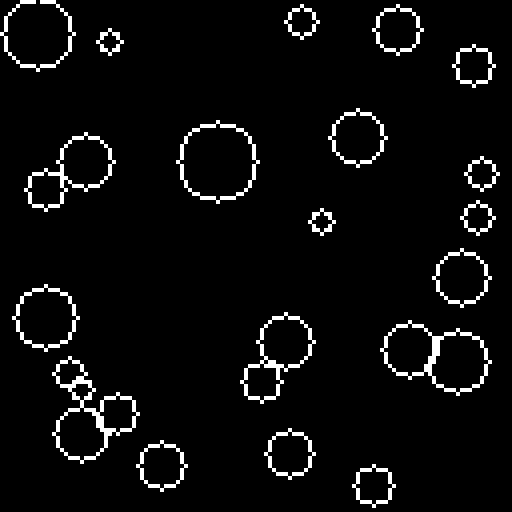
\includegraphics[width=0.25\textwidth]{img/cg_content_25.png} }}%
    \qquad
    \subfloat[synthesised]{{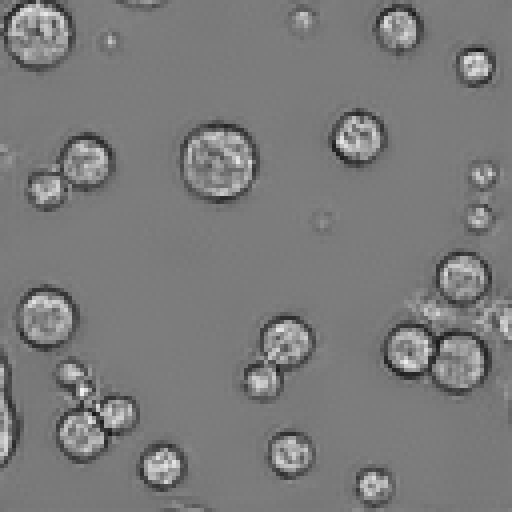
\includegraphics[width=0.25\textwidth]{img/cg_fake_a_25.png} }}%
    \qquad
    \subfloat[reconstructed]{{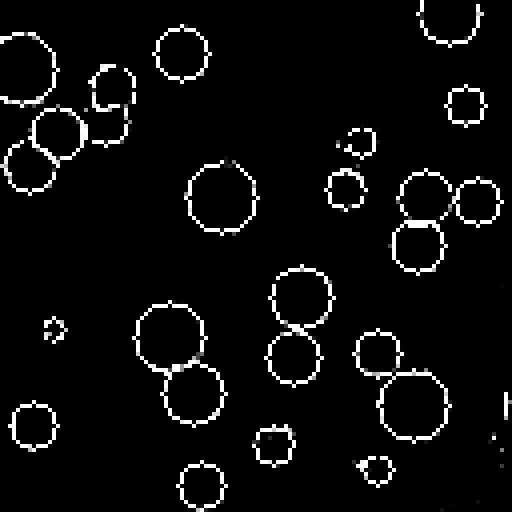
\includegraphics[width=0.25\textwidth]{img/cg_recon_b_25.png} }}
    \qquad
    \subfloat[content]{{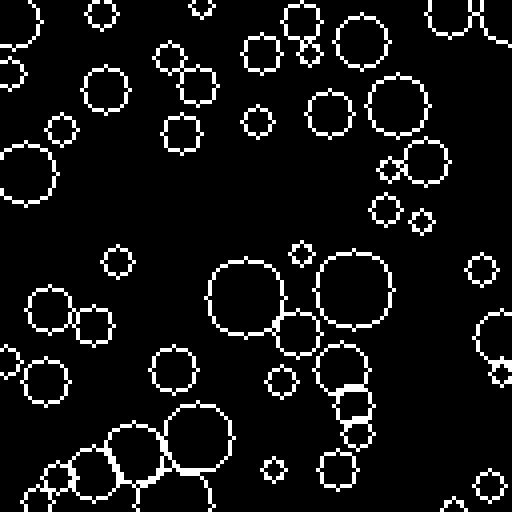
\includegraphics[width=0.25\textwidth]{img/cg_content_50.png} }}%
    \qquad
    \subfloat[synthesised]{{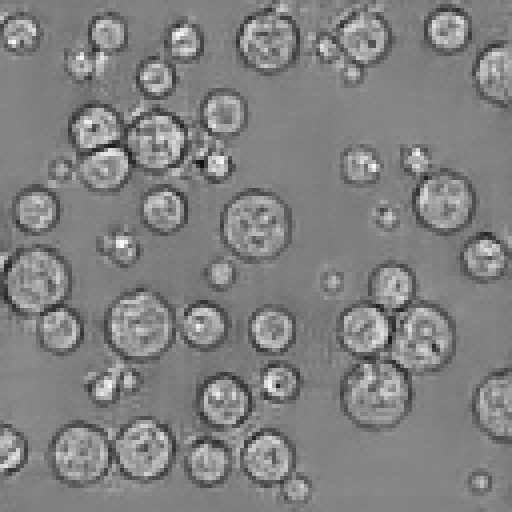
\includegraphics[width=0.25\textwidth]{img/cg_fake_a_50.png} }}%
    \qquad
    \subfloat[reconstructed]{{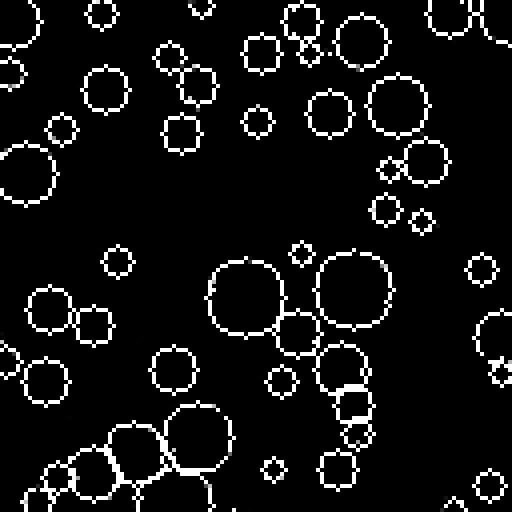
\includegraphics[width=0.25\textwidth]{img/cg_recon_b_50.png} }}
    \qquad
    \subfloat[content]{{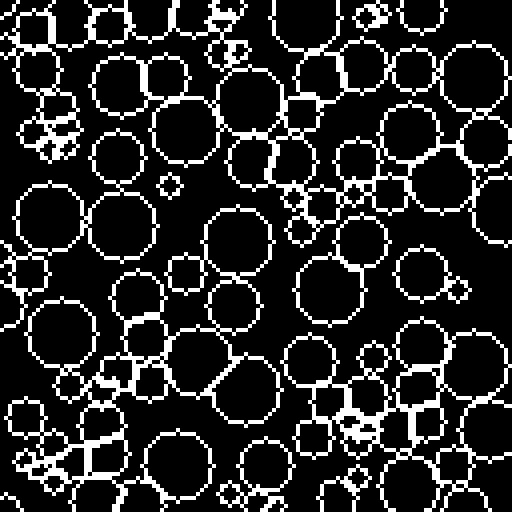
\includegraphics[width=0.25\textwidth]{img/cg_content_100.png} }}%
    \qquad
    \subfloat[synthesised]{{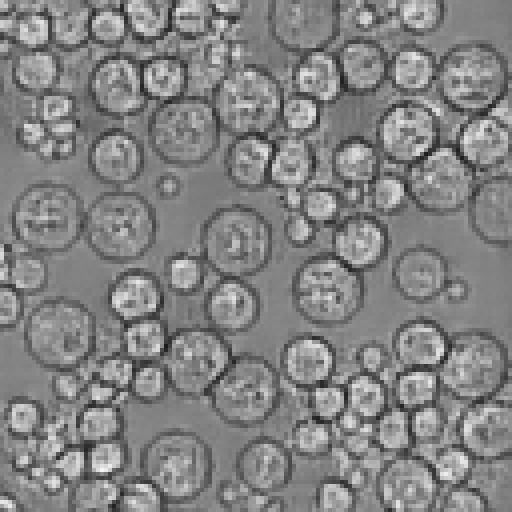
\includegraphics[width=0.25\textwidth]{img/cg_fake_a_100.png} }}%
    \qquad
    \subfloat[reconstructed]{{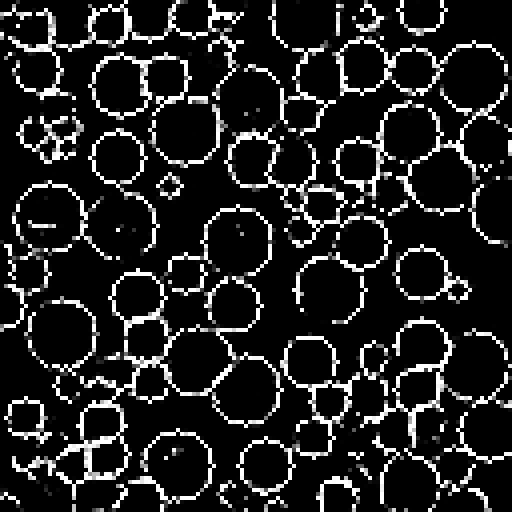
\includegraphics[width=0.25\textwidth]{img/cg_recon_b_100.png} }}
    \qquad
    \subfloat[content]{{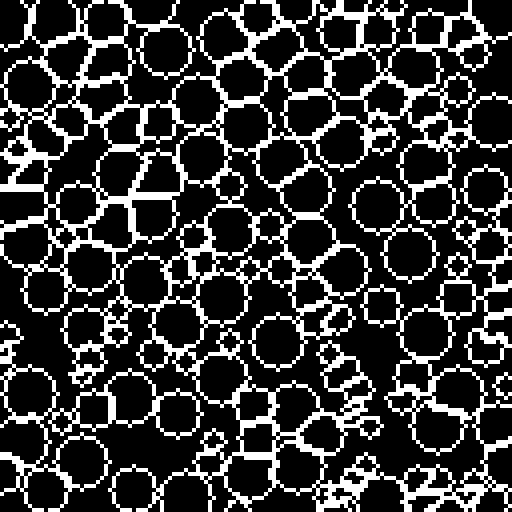
\includegraphics[width=0.25\textwidth]{img/cg_content_150.png} }}%
    \qquad
    \subfloat[synthesised]{{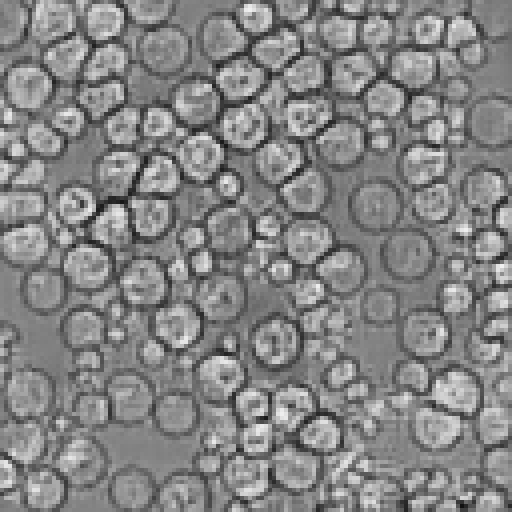
\includegraphics[width=0.25\textwidth]{img/cg_fake_a_150.png} }}%
    \qquad
    \subfloat[reconstructed]{{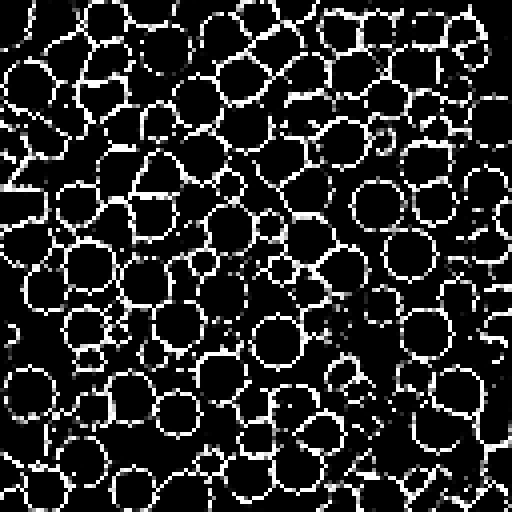
\includegraphics[width=0.25\textwidth]{img/cg_recon_b_150.png} }}
    \qquad
    \caption{Examples of CycleGAN generated images. Columns organised with content specification input image $X$ (left), $G(X)$ generated image (center) and reconstruction $F(G(X))$ (right). The number of cells are increased over the rows: $25$, $50$, $100$, and $150$.}%
    \label{fig:first_results_cycle_gans}%
\end{figure}

\section{Fine-tuning a state-of-the art object detection system}
\label{sec:fine_tuning_rcnn}

With the content-to-style generator from Section \ref{subsec:first_results_cyclegans} acting as an ``oracle'' for perfectly-annotated training data, a state-of-the-art object detection system may be trained, such as that which remained elusive in Chapter \ref{Chapter5}. The Faster R-CNN model (\cite{girshick2015fast}) is chosen for this task. A full discussion of the RCNN series of object detectors is available in Section \ref{subsec:rcnn_definition}. The Faster RCNN implementation available in the PyTorch framework (\cite{paszke2017automatic}) is used. This has been pretrained on the COCO object detection dataset \cite{lin2014microsoft}. A simple fine-tuning procedure is to replace the classification and bounding box regression ``heads'' of the network, that is, leaving the backbone and region proposal network untouched, and to continue gradient descent on the new data with a lowered learning rate. This is done, with a learning rate of $10^{-4}$, training with SGD with momentum. Mini-batches are formed for training with $8$ synthetic images. The (perfect) bounding box annotation (and, in principle, object class information) is determined by the drawing procedure of the synthetic image.

\begin{figure}[h]%
    \centering
    \subfloat[Weakly supervised training set]{{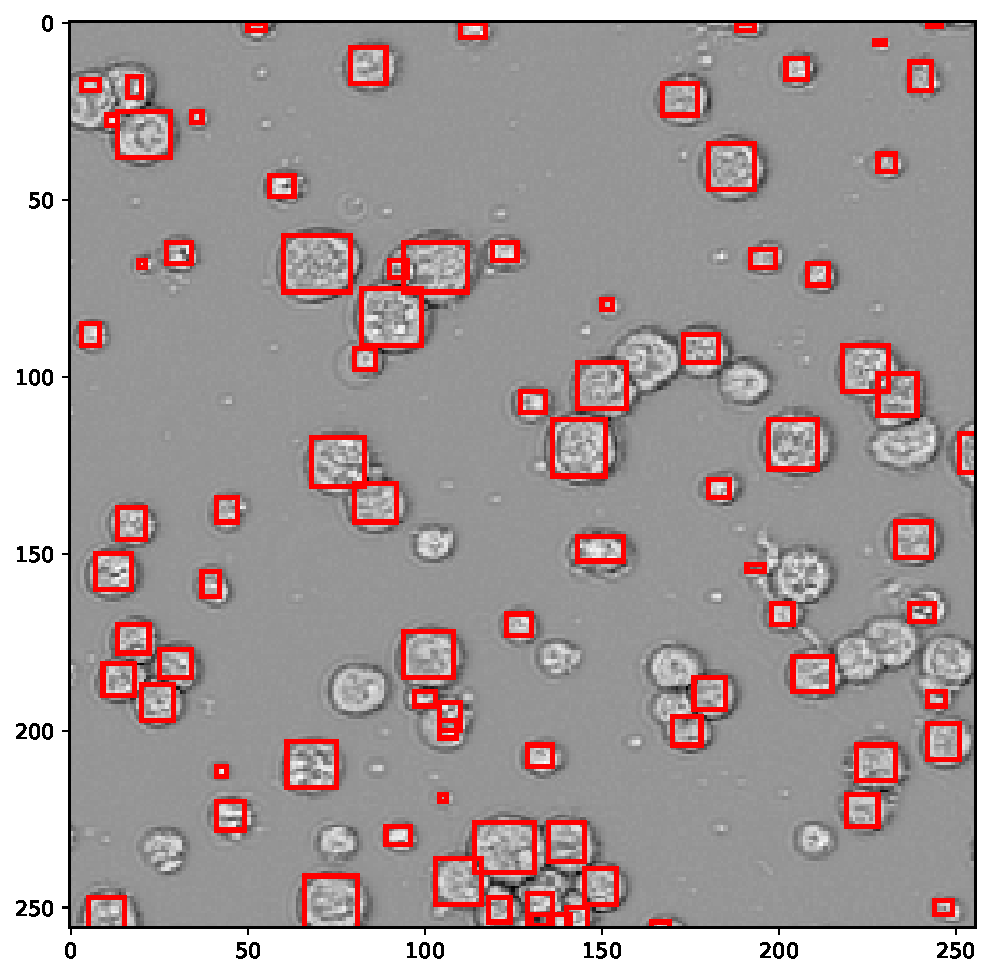
\includegraphics[width=0.45\textwidth]{img/rcnn_weak.pdf} }}%
    \qquad
    \subfloat[Synthetic training set]{{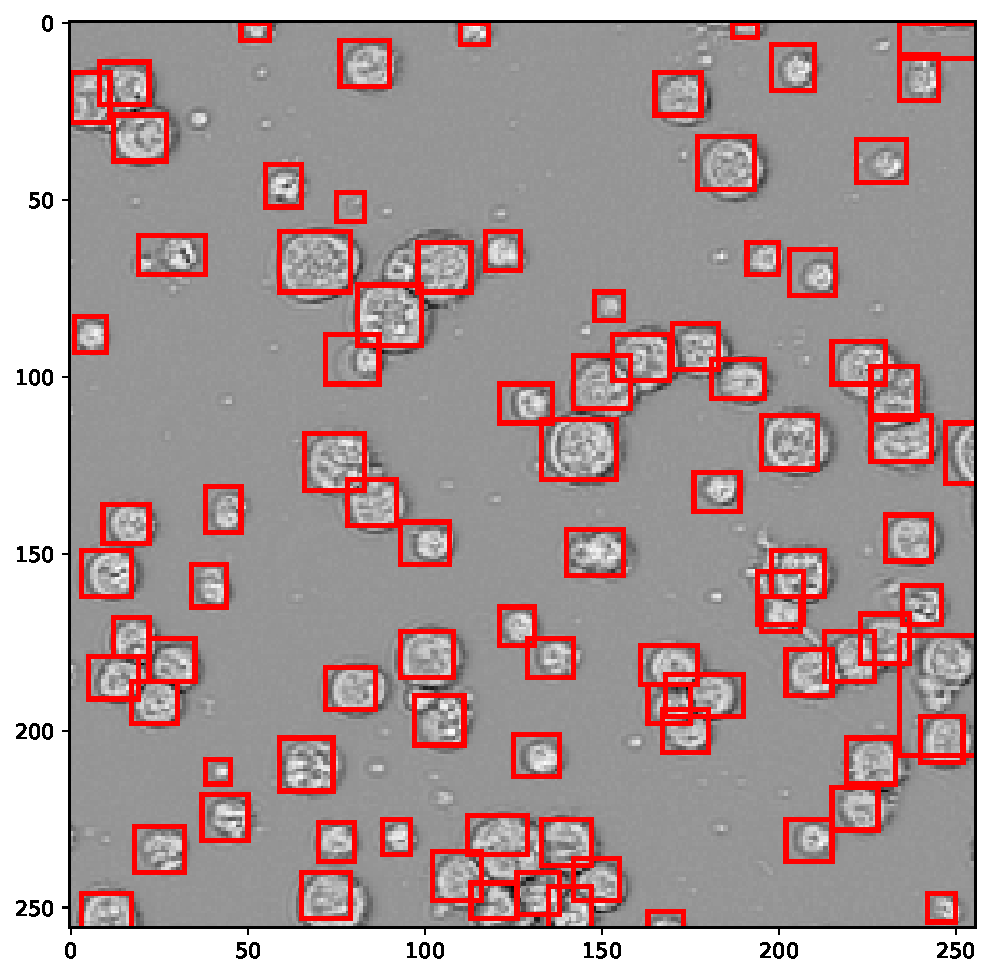
\includegraphics[width=0.45\textwidth]{img/rcnn_synthetic.pdf} }}%
    \caption{Comparison of outcomes of Faster R-CNN on a test image when a) fine-tuned on a weakly supervised dataset and b) fine-tuned on synthetic images.}%
    \label{fig:faster_rcnn}%
\end{figure}

The outcome of this fine-tuning is a detection system capable of detecting cells (but not classification, for now). A comparison is made between Faster R-CNN trained on the CycleGAN synthetic images against the incomplete annotations arising from the automatic pipeline proposed in Section \ref{subsec:object_detection_data}. Recall, the argument for pursuing a custom detector in Chapter \ref{Chapter5} was that such a \emph{weakly supervised} dataset would be insufficient for training a state-of-the-art system like Faster R-CNN. We see in Figure \ref{fig:faster_rcnn} evidence to support this intuition, in which are compared the outcomes of the fine-tuned R-CNN on an authentic test image, when fine-tuned first on a weakly supervised dataset, then on the CycleGAN-generated images.

\section{Perspectives on synthesising a full object detection dataset}
\label{sec:full_object_detection_dataset}
In Section \ref{sec:fine_tuning_rcnn} the viability of training a state-of-the art object detection system on fully-annotated synthetic images has been shown. The missing component is to incorporate classification into the framework. In principle, the R-CNN detector is designed to learn this task simultaneously with the object detection, however, the CycleGANs, being a fully unsupervised model have no means for injecting this information into the data-generating process. Clearly, one could use the R-CNN as a region proposal algorithm and classify regions with a separately trained classifier (such as in Section \ref{subsec:training}). Preliminary results with this approach demonstrate this is a viable approach. However, the R-CNN system should be altogether more powerful if trained on a full annotation of object class and location. One could, alternatively, attempt to incorporate the weakly annotated ground truth (as utilised in Section \ref{sec:fine_tuning_rcnn}) into the R-CNN fine-tuning in an attempt to teach it about Raji cell classes.

In the following, however, an extension to the CycleGAN system above is conceptualised that would be theoretically capable of providing both a complete annotation of synthesised images, encompassing both object localisation and class annotations. This extension takes the form of an additional discriminator for the content-to-style generator, that, in contrast to the PatchGAN discriminator, discriminates on regions of interest. Such a \emph{region of interest discriminator}, $D_{roi}$ compares fake cells localised by bounding boxes inside generated images with a pre-cropped ``library'' of real cells. The library can include class information for the individual crops, which can be combined in the fashion of a conditional GAN. The content image would also have to encode class information in some way (for example, by intensity or a one-hot encoding). Thus, the $D_{roi}$ discriminator could provide a mechanism to enforce class information at the resolution of specific regions of interest. For a preliminary implementation of this idea, see Appendix \ref{sec:training_roi_classifier}.

\subsection{Region of interest discrimination}

Let us define an auxiliary discriminator for image-to-image GANs,

\begin{equation}
d_{roi} : X, B \to \{0, 1\},
\end{equation}

for image domain $X$ and bounding box domain $B$, with $d_{roi}(\mathbf{x}, b) = d(\rho(f(\mathbf{x}), b))$, for input image $\mathbf{x} \sim X$, bounding box $b \sim B$, and where we conceive of a neural network comprising of feature extraction layers $f$, classification layers $d$, and separated by RoIPool layer $\rho$. A RoIPool layer\footnote{See also RoIAlign layer (\cite{he2017mask})} (\cite{girshick2015fast}) generalises the MaxPooling layer and quantises regions of interest (RoIs) into a fixed size,

\begin{equation}
\rho : X, B \to \mathbf{y},
\end{equation}

for input tensor $\mathbf{x} \in \mathbb{R}^{1\times W \times H \times C}$, set of $K$ bounding box tuples $B$, and tensor output $\mathbf{y} \in \mathbb{R}^{K \times w \times h \times C}$ with quantised dimensions $w < W$ and $h < H$. To clarify, the incoming tensor $\mathbf{x}$ is transformed into a ``pseudo-batch'' of $K$ tensors for the $K$ bounding boxes of $B$. Akin to the PatchGAN (see Section \ref{subsec:image_to_image}), the full discriminator output averages over the individual bounding boxes,

\begin{equation}
D_{roi} = \frac{1}{|\mathcal{B}(\mathbf{x})|}\sum_{b \in \mathcal{B}(\mathbf{x})} d_{roi}(\mathbf{x}, b),
\end{equation}

where the operator $\mathcal{B}$ returns the set of bounding boxes of image $\mathbf{x}$. Of course, in the present case, the bounding boxes are decided in advance by virtue of drawing the content images. This is trained in the loss function,

\begin{equation}
\max_{G, F}\min_{D_X, D_Y, D_{roi}} \mathcal{L}_{CG} + \mathcal{L}_{GAN}(D_{roi}, G, X, Y),
\end{equation}

where $\mathcal{L}_{CG}$ is the CycleGAN loss function defined in Equation \ref{eq:cycle_gan}. The setup is illustrated in Figure \ref{fig:roi_gan}. Just like the contour generation, the problem of obtaining a crop library will vary from problem to problem. In this instance, however, direct access to such a library comes from the automatic procedure described in Section \ref{subsec:object_detection_data}. Some basic proofs of concept of using the RoIPool for classification and GAN discrimination are given in Appendix \ref{sec:training_roi_classifier}.

\begin{figure}[h]
\centering
\tikzset{every picture/.style={line width=0.75pt}} %set default line width to 0.75pt        

\begin{tikzpicture}[x=0.75pt,y=0.75pt,yscale=-1,xscale=1]
%uncomment if require: \path (0,437); %set diagram left start at 0, and has height of 437

%Image [id:dp32316243876461437] 
\draw (310,30) node  {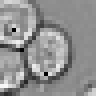
\includegraphics[width=15pt,height=15pt]{img/roi_gan_cell_5703.png}};
%Shape: Square [id:dp13954798751068864] 
\draw  [color={rgb, 255:red, 0; green, 0; blue, 0 }  ,draw opacity=1 ][line width=0.75]  (300,20) -- (320,20) -- (320,40) -- (300,40) -- cycle ;

%Image [id:dp8299615438651444] 
\draw (260,30) node  {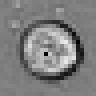
\includegraphics[width=15pt,height=15pt]{img/roi_gan_cell_28511.png}};
%Shape: Square [id:dp6339166487175822] 
\draw  [color={rgb, 255:red, 0; green, 0; blue, 0 }  ,draw opacity=1 ][line width=0.75]  (250,20) -- (270,20) -- (270,40) -- (250,40) -- cycle ;

%Image [id:dp27154181356436824] 
\draw (230,30) node  {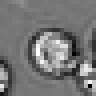
\includegraphics[width=15pt,height=15pt]{img/roi_gan_cell_33686.png}};
%Shape: Square [id:dp2864387695737485] 
\draw  [color={rgb, 255:red, 0; green, 0; blue, 0 }  ,draw opacity=1 ][line width=0.75]  (220,20) -- (240,20) -- (240,40) -- (220,40) -- cycle ;

%Image [id:dp5350014141118905] 
\draw (270,160) node  {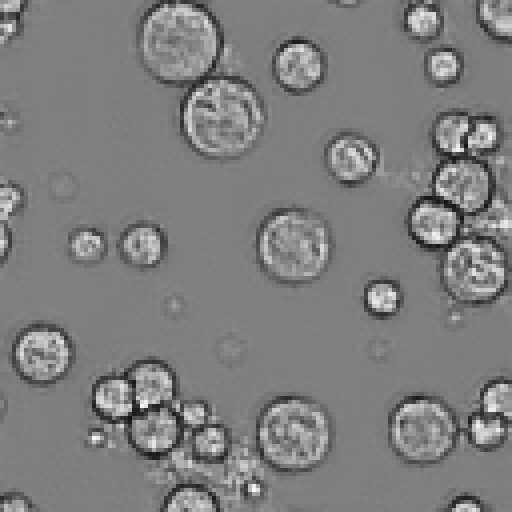
\includegraphics[width=90pt,height=90pt]{img/roi_gan_fake_a.png}};
%Shape: Square [id:dp5178016203350967] 
\draw   (20,100) -- (140,100) -- (140,220) -- (20,220) -- cycle ;
%Shape: Square [id:dp7106552529782532] 
\draw   (210,100) -- (330,100) -- (330,220) -- (210,220) -- cycle ;
%Shape: Square [id:dp8330459711802627] 
\draw   (210,250) -- (330,250) -- (330,370) -- (210,370) -- cycle ;
%Shape: Square [id:dp21278621661100205] 
\draw  [color={rgb, 255:red, 0; green, 0; blue, 0 }  ,draw opacity=1 ][line width=0.75]  (252,118) -- (272,118) -- (272,138) -- (252,138) -- cycle ;
%Shape: Square [id:dp9867797884989475] 
\draw  [color={rgb, 255:red, 0; green, 0; blue, 0 }  ,draw opacity=1 ][line width=0.75]  (302,142) -- (322,142) -- (322,162) -- (302,162) -- cycle ;
%Shape: Square [id:dp5415469187486135] 
\draw  [color={rgb, 255:red, 0; green, 0; blue, 0 }  ,draw opacity=1 ][line width=0.75]  (269,148) -- (289,148) -- (289,168) -- (269,168) -- cycle ;
%Straight Lines [id:da6425394215304491] 
\draw [color={rgb, 255:red, 0; green, 0; blue, 0 }  ,draw opacity=1 ][line width=0.75]    (140,160) -- (158,160) ;
\draw [shift={(160,160)}, rotate = 180] [color={rgb, 255:red, 0; green, 0; blue, 0 }  ,draw opacity=1 ][line width=0.75]    (10.93,-3.29) .. controls (6.95,-1.4) and (3.31,-0.3) .. (0,0) .. controls (3.31,0.3) and (6.95,1.4) .. (10.93,3.29)   ;
%Straight Lines [id:da5543481152981689] 
\draw [color={rgb, 255:red, 0; green, 0; blue, 0 }  ,draw opacity=1 ][line width=0.75]    (330,310) -- (379.28,181.87) ;
\draw [shift={(380,180)}, rotate = 471.04] [color={rgb, 255:red, 0; green, 0; blue, 0 }  ,draw opacity=1 ][line width=0.75]    (10.93,-3.29) .. controls (6.95,-1.4) and (3.31,-0.3) .. (0,0) .. controls (3.31,0.3) and (6.95,1.4) .. (10.93,3.29)   ;
%Straight Lines [id:da2524733821298324] 
\draw [color={rgb, 255:red, 0; green, 0; blue, 0 }  ,draw opacity=1 ][fill={rgb, 255:red, 255; green, 255; blue, 255 }  ,fill opacity=1 ][line width=0.75]    (322,142) -- (379.01,41.74) ;
\draw [shift={(380,40)}, rotate = 479.62] [color={rgb, 255:red, 0; green, 0; blue, 0 }  ,draw opacity=1 ][line width=0.75]    (10.93,-3.29) .. controls (6.95,-1.4) and (3.31,-0.3) .. (0,0) .. controls (3.31,0.3) and (6.95,1.4) .. (10.93,3.29)   ;
%Straight Lines [id:da5549136324649655] 
\draw [color={rgb, 255:red, 0; green, 0; blue, 0 }  ,draw opacity=1 ][fill={rgb, 255:red, 255; green, 255; blue, 255 }  ,fill opacity=1 ][line width=0.75]    (271,119) -- (358.5,41.33) ;
\draw [shift={(360,40)}, rotate = 498.41] [color={rgb, 255:red, 0; green, 0; blue, 0 }  ,draw opacity=1 ][line width=0.75]    (10.93,-3.29) .. controls (6.95,-1.4) and (3.31,-0.3) .. (0,0) .. controls (3.31,0.3) and (6.95,1.4) .. (10.93,3.29)   ;
%Straight Lines [id:da35650961790429714] 
\draw [color={rgb, 255:red, 0; green, 0; blue, 0 }  ,draw opacity=1 ][fill={rgb, 255:red, 255; green, 255; blue, 255 }  ,fill opacity=1 ][line width=0.75]    (290,150) -- (368.82,41.62) ;
\draw [shift={(370,40)}, rotate = 486.03] [color={rgb, 255:red, 0; green, 0; blue, 0 }  ,draw opacity=1 ][line width=0.75]    (10.93,-3.29) .. controls (6.95,-1.4) and (3.31,-0.3) .. (0,0) .. controls (3.31,0.3) and (6.95,1.4) .. (10.93,3.29)   ;
%Image [id:dp735349159455305] 
\draw (270,310) node  {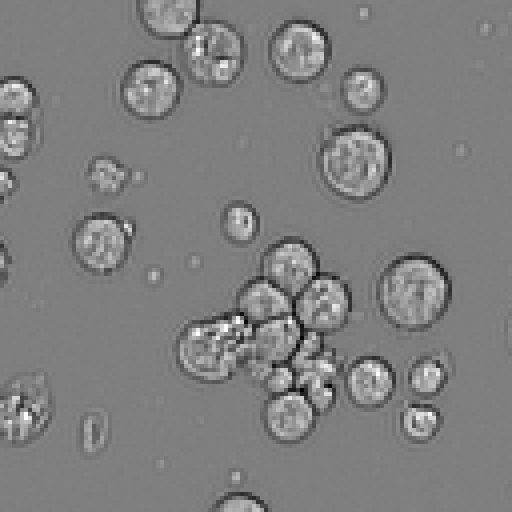
\includegraphics[width=90pt,height=90pt]{img/roi_gan_style_img.png}};
%Straight Lines [id:da4101426865259086] 
\draw [color={rgb, 255:red, 0; green, 0; blue, 0 }  ,draw opacity=1 ][line width=0.75]    (180,160) -- (198,160) ;
\draw [shift={(200,160)}, rotate = 180] [color={rgb, 255:red, 0; green, 0; blue, 0 }  ,draw opacity=1 ][line width=0.75]    (10.93,-3.29) .. controls (6.95,-1.4) and (3.31,-0.3) .. (0,0) .. controls (3.31,0.3) and (6.95,1.4) .. (10.93,3.29)   ;
%Straight Lines [id:da13339117808681678] 
\draw [color={rgb, 255:red, 0; green, 0; blue, 0 }  ,draw opacity=1 ][line width=0.75]    (330,160) -- (348,160) ;
\draw [shift={(350,160)}, rotate = 180] [color={rgb, 255:red, 0; green, 0; blue, 0 }  ,draw opacity=1 ][line width=0.75]    (10.93,-3.29) .. controls (6.95,-1.4) and (3.31,-0.3) .. (0,0) .. controls (3.31,0.3) and (6.95,1.4) .. (10.93,3.29)   ;
%Straight Lines [id:da27531765046490264] 
\draw [color={rgb, 255:red, 0; green, 0; blue, 0 }  ,draw opacity=1 ][line width=0.75]    (410,160) -- (428,160) ;
\draw [shift={(430,160)}, rotate = 180] [color={rgb, 255:red, 0; green, 0; blue, 0 }  ,draw opacity=1 ][line width=0.75]    (10.93,-3.29) .. controls (6.95,-1.4) and (3.31,-0.3) .. (0,0) .. controls (3.31,0.3) and (6.95,1.4) .. (10.93,3.29)   ;
%Straight Lines [id:da7100088338531173] 
\draw [color={rgb, 255:red, 0; green, 0; blue, 0 }  ,draw opacity=1 ][line width=0.75]    (410,30) -- (428,30) ;
\draw [shift={(430,30)}, rotate = 180] [color={rgb, 255:red, 0; green, 0; blue, 0 }  ,draw opacity=1 ][line width=0.75]    (10.93,-3.29) .. controls (6.95,-1.4) and (3.31,-0.3) .. (0,0) .. controls (3.31,0.3) and (6.95,1.4) .. (10.93,3.29)   ;
%Straight Lines [id:da35382637692965624] 
\draw [color={rgb, 255:red, 0; green, 0; blue, 0 }  ,draw opacity=1 ][line width=0.75]  [dash pattern={on 4.5pt off 4.5pt}]  (140,220) -- (140,400) ;
%Straight Lines [id:da25520328990920704] 
\draw [color={rgb, 255:red, 0; green, 0; blue, 0 }  ,draw opacity=1 ][line width=0.75]  [dash pattern={on 4.5pt off 4.5pt}]  (140,400) -- (400,400) ;
%Straight Lines [id:da6043367006130822] 
\draw [color={rgb, 255:red, 0; green, 0; blue, 0 }  ,draw opacity=1 ][line width=0.75]  [dash pattern={on 4.5pt off 4.5pt}]  (400,400) -- (400,182) ;
\draw [shift={(400,180)}, rotate = 450] [color={rgb, 255:red, 0; green, 0; blue, 0 }  ,draw opacity=1 ][line width=0.75]    (10.93,-3.29) .. controls (6.95,-1.4) and (3.31,-0.3) .. (0,0) .. controls (3.31,0.3) and (6.95,1.4) .. (10.93,3.29)   ;
%Image [id:dp5129295451379209] 
\draw (80,160) node  {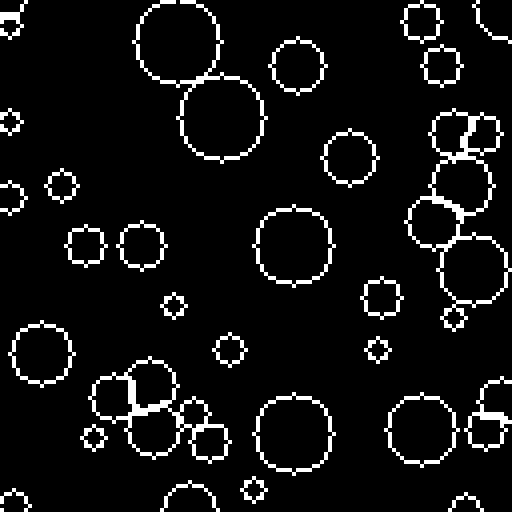
\includegraphics[width=90pt,height=90pt]{img/roi_gan_input_img.png}};
%Straight Lines [id:da9036519529480025] 
\draw [color={rgb, 255:red, 0; green, 0; blue, 0 }  ,draw opacity=1 ][line width=0.75]    (330,30) -- (348,30) ;
\draw [shift={(350,30)}, rotate = 180] [color={rgb, 255:red, 0; green, 0; blue, 0 }  ,draw opacity=1 ][line width=0.75]    (10.93,-3.29) .. controls (6.95,-1.4) and (3.31,-0.3) .. (0,0) .. controls (3.31,0.3) and (6.95,1.4) .. (10.93,3.29)   ;

% Text Node
\draw (81,239.5) node  [font=\scriptsize] [align=left] {Content image};
% Text Node
\draw (271.5,382.5) node  [font=\scriptsize] [align=left] {Real image};
% Text Node
\draw (270.5,232.5) node  [font=\scriptsize] [align=left] {Fake image};
% Text Node
\draw (454,157.5) node  [font=\scriptsize] [align=left] {Real/fake};
% Text Node
\draw (454,27.5) node  [font=\scriptsize] [align=left] {Real/fake};
% Text Node
\draw (272,417.5) node  [font=\scriptsize] [align=left] {(Conditional)};
% Text Node
\draw (170.5,156.5) node  [font=\large] [align=left] {$\displaystyle G$};
% Text Node
\draw (383,156.5) node  [font=\large] [align=left] {$\displaystyle D_{Patch}$};
% Text Node
\draw (381,26.5) node  [font=\large] [align=left] {$\displaystyle D_{RoI}$};
% Text Node
\draw (271,52.5) node  [font=\scriptsize] [align=left] {Crop library};
% Text Node
\draw (274,22) node [anchor=north west][inner sep=0.75pt]   [align=left] {$\displaystyle \cdot \cdot \cdot $};
\end{tikzpicture}

\caption{Conceptualisation of an extension to adversarial image-to-image translation networks with a region of interest discriminator $D_{roi}$. The $D_{roi}$ relies on a library of real crops to compare to cells synthesised by $G$ in the prescribed regions of the content image.}
\label{fig:roi_gan}
\end{figure}

\section{Discussion}

This chapter illustrated the viability for the synthesis of images of cells based on phase contrast images of CAR-T experiments. This was shown both at the level of single cells with convolutional and conditional GANs in Section \ref{sec:feasibility_synthesising}, and at the population level through applications of style transfer both classical (Section \ref{subsec:style_transfer_application}) and with CycleGANs (Section \ref{sec:cycle_gans}). Generating populations of cells according to a content image ``blueprint'' proves to be a powerful way of generating complete annotations in an entirely unsupervised way, sufficient to train a state-of-the-art object detection system (Section \ref{sec:fine_tuning_rcnn}). The blueprint (Section  \ref{subsec:conditional_dilation}) models various characteristics of individual cells and groups of cells in order to facilitate the style transfer. A means for incorporating class information was also conceptualised in Section \ref{sec:full_object_detection_dataset} as a full realisation of the concept of unsupervised training data creation for the phenotyping of CAR-T experiments.

At least two aspects of the current pipeline can be improved. The first is the blueprint content image, which, as of yet, does not account for the tendency of Raji cells to cluster. As mentioned previously, this is a matter of changing the distribution of cell placement in the blueprint from uniform random placement. The second is to finalise the inclusion of class information in the training set synthesis. A concept was proposed in Section \ref{sec:full_object_detection_dataset}, with a number of alternatives also outlined.
